\part{Quantum statistical mechanics}

\chapter{Quantum Mechanics}

    In this chapter, we will recall some basic notion of quantum mechanics: starting from general definitions of states, equations of motion, observables, time evolution and investigating the formalism of density matrices and the difference between pure quantum and classical mixed states.

\section{States and projectors}

    In quantum mechanics, a pure state of a quantum particle is represented by a normalised vector in a (separable) Hilbert space $\ket{\psi} \in \mathcal H$. This is the best knowledge we can have. An Hilbert space $\mathcal H$ is a vector space on $\mathbb C$, i.e.~in which a linear superposition of vectors is still in the space 
    \begin{equation*}
        \lambda \ket{\psi} + \mu \ket{\phi} \in \mathcal H ~, \quad \forall \ket{\psi}, \ket{\phi} \in \mathcal H ~, \forall \lambda, \mu \in \mathbb C ~, 
    \end{equation*}
    endowed with a scalar product $\braket{\psi}{\phi}$. In particular, via the scalar product, it is possible to associate a norm to the state, which is set to $1$ by the probability interpretation $||\psi||^2 = \braket{\psi}{\psi} = 1$. In the Schroedinger representation, this means that the wave function is a square-integrable function $\psi(t,\mathbf x) \in L^2(\mathbb R^d)$. Furthermore, the probability interpretation tells us that $|\psi(t, \mathbf x)|$ is the probability density to find the particle in a volume element $d^d x$ at time $t$ and the normalisation condition that the total probability to find the particle in the whole $\mathbb R^d$ is $1$ 
    \begin{equation*}
        \int_{\mathbb R^d} d^d x ~ |\psi(t,x)|^2 = 1 ~.
    \end{equation*}
    However, because of that, a state is not associated to a single vector, but to a class of equivalence of them, called a ray in the Hilbert space. This is true since two states are physically equivalent if $\ket{\psi'} = \exp(i \varphi) \ket{\psi}$, because their norms are the same. To remove this ambiguity, we introduce the notion of projection operators or projectors, that uniquely determine a state, 
    \begin{equation*}
        P_\psi = \frac{\ket{\psi} \bra{\psi}}{\braket{\psi}{\psi}} ~,
    \end{equation*}
    which for normalisation states becomes 
    \begin{equation}\label{proj}
        P_\psi = \ket{\psi} \bra{\psi} ~.
    \end{equation}
    \begin{proof}
        If $\ket{\psi'} = \exp(i \varphi) \ket{\psi}$ and $\bra{\psi'} = \exp(- i \varphi) \bra{\psi}$, we have 
        \begin{equation*}
            P_{\psi'} = \ket{\psi'} \bra{\psi'} = \cancel{\exp(i \varphi)} \ket{\psi} \cancel{\exp(- i \varphi)} \bra{\psi} = \ket{\psi} \bra{\psi} = P_\psi ~.
        \end{equation*}
    \end{proof}

    It projects onto the $1$-dimensional subspace $\mathcal H_\psi = \{\lambda \ket{\psi} \colon \lambda \in \mathbb C\}$ generated by the state $\ket{\psi}$
    \begin{equation*}
        P_\psi \colon \mathcal H \rightarrow \mathcal H_\psi ~.
    \end{equation*}
    \begin{proof}
        In fact, $\forall \ket{\phi} \in \mathcal H$, we decomposed the Hilbert space into the direct orthogonal sum of the subspace spanned by $\mathcal H_{\psi}$ and its orthogonal complement $\mathcal H^\perp$:
        \begin{equation*}
            \ket{\phi} = \alpha \ket{\psi} + \beta \ket{\psi^\perp} ~,
        \end{equation*}
        where $\ket{\psi} \in \mathcal H_\psi$, $\ket{\psi^\perp} \in \mathcal H^\perp$ and $\braket{\psi}{\psi^\perp} = 0$. Therefore, the action of the projector is
        \begin{equation*}
            P_\psi \ket{\phi} = \alpha P_\psi \ket{\psi} + \beta P_\psi \ket{\psi^\perp} = \alpha \ket{\psi} \underbrace{\braket{\psi}{\psi}}_1 + \beta \ket{\psi} \underbrace{\braket{\psi}{\psi^\perp}}_0 = \alpha \ket{\psi} \in \mathcal H_\psi ~.
        \end{equation*}
    \end{proof}
    Moreover, since projectors are orthogonal, we can define the projector onto the orthogonal subspace as $P_\psi^\perp = \mathbb I - P_\psi$ such that it satisfies $P_\psi P_\psi^\perp = P_\psi^\perp P_\psi = 0$. This can be generalised for a generic set of orthogonal subspaces. In fact, given an orthonormal basis $\{\ket{e_n}\}$, a projector onto an element of this basis is $P_n = \ket{e_n} \bra{e_n}$ and the orthonormality condition reads as $P_n P_m = P_m P_n = 0$ for $n \neq m$. Projectors satisfy the following properties 
    \begin{enumerate}
        \item boundness, i.e. 
            \begin{equation*}
                ||P_\psi|| < \infty~,
            \end{equation*}
        \item hermiticity, i.e. 
            \begin{equation*}
                P_\psi^\dagger = P_\psi ~,
            \end{equation*}
        \item idempotence, i.e. 
            \begin{equation}\label{idem}
                P_\psi^2 = P_\psi ~,
            \end{equation}
        \item positive defined, i.e. $\forall \ket{\phi} \in \mathcal H$
            \begin{equation*}
                \bra{\phi} P_\psi \ket{\phi} \geq 0 ~,
            \end{equation*}
        \item trace equals to $1$, i.e. 
            \begin{equation*}
                \tr P_\psi = 1 ~.
            \end{equation*}
    \end{enumerate}
    Actually, there is a theorem that ensures that an operator, such that it satifies these 5 conditions, is indeed a projectors.
    \begin{proof}
        For the boundness, $\forall \ket{\phi} \in \mathcal H$
        \begin{equation*}
            ||P_\psi \ket{\phi}||^2 = \bra{\phi} P_\psi^\dagger P_\psi \ket{\phi} = \braket{\phi}{\psi} \underbrace{\braket{\psi}{\psi}}_1 \braket{\psi}{\phi} = |\braket{\psi}{\phi}|^2 \leq ||\phi||^1 ~,
        \end{equation*}
        hence,
        \begin{equation*}
            ||P_\psi|| = \frac{||P_\psi \ket{\phi}||}{||\phi||} \leq 1 ~.
        \end{equation*}
        For the hermiticity
        \begin{equation*}
            P_\psi^\dagger = (\ket{\psi} \bra{\psi})^\dagger = \bra{\psi}^\dagger \ket{\psi}^\dagger = \ket{\psi} \bra{\psi} = P_\psi ~.
        \end{equation*}
        For the idempotence
        \begin{equation*}
            P_\psi^2 = (\ket{\psi} \bra{\psi})^2 = \ket{\psi} \underbrace{\braket{\psi}{\psi}}_1 \bra{\psi} = \ket{\psi} \bra{\psi} = P_\psi ~.
        \end{equation*}
        For the positive definedness 
        \begin{equation*}
            \bra{\phi} P_\psi \ket{\phi} = \braket{\phi}{\psi} \braket{\psi}{\phi} = |\braket{\psi}{\phi}|^2 \geq 0 ~.
        \end{equation*}
        For the trace, since it is independent from the choice of the basis, we choose $\ket{\psi} = \ket{\psi_1}$ such that $\braket{\psi}{\psi_n} = \delta_{n,1}$ and 
        \begin{equation*}
            \tr P_\psi = \sum_{n=0}^{\infty} \bra{\psi_n} P_\psi \ket{\psi_n} = \sum_{n=0}^{\infty} \underbrace{\braket{\psi_n}{\psi}}_{\delta_{n,1}} \braket{\psi}{\psi_n} = \sum_{n=0}^{\infty} \underbrace{\delta_{n,1}}_{n=1} \braket{\psi}{\psi_n} = \braket{\psi}{\psi_1} = \braket{\psi_1}{\psi_1} = 1 ~.
        \end{equation*}
    \end{proof}

    Given an orthonormal basis $\{\ket{e_n}\}_{n=1}^\infty$ of a separable Hilbert space, the trace is defined as 
    \begin{equation*}
        \tr A = \sum_{n=1}^\infty A_{nn} = \sum_{n=1}^\infty \bra{e_n} A \ket{e_n} ~.
    \end{equation*}
    It may happen that this series is not convergent. If it is convergent, the operator $A$ is called a trace-class operator. Furthermore, if it is absolute convergent, the trace is independent on the choice of the basis. Recall that in the finite-dimensional case, the trace of a matrix is always convergent and independent on the choice of the basis.

\section{Observables and time evolution}

    An observable is a linear hermitian operator $\hat A$ acting on the Hilbert space. We require the self-adjointness because, by the spectral theorem, they are always diagonalisable with a positive spectrum. This means that its eigenvalues are real and it always admits an orthonormal eigenbasis $\{\ket{\psi_n}\}$
    \begin{equation}\label{eigen}
        A \ket{\psi_n} = \lambda_n \ket{\psi_n} ~,
    \end{equation}
    where $\lambda_n \in \mathbb R$. In this way, $\forall \ket{\phi} \in \mathcal H$, we can expand it into the eigenbasis 
    \begin{equation}\label{exp}
        \ket{\phi} = \sum_{n=1}^{\infty} c_n \ket{\psi_n} ~,
    \end{equation}
    where $c_n \in \mathbb C$.
    Eigenprojectors, defined as 
    \begin{equation*}
        P_n = \ket{\psi_n} \bra{\psi_n} ~,
    \end{equation*}
    satisfy the following properties 
    \begin{enumerate}
        \item self-adjointness, i.e.
            \begin{equation*}
                P_n^\dagger = P_n ~,
            \end{equation*}
        \item orthonormality, i.e.
            \begin{equation*}
                P_n P_m = \delta_{nm} P_n ~,
            \end{equation*}
        \item completeness relation, i.e.
            \begin{equation}\label{compl}
                \sum_{n = 0}^{\infty} P_n = \mathbb I~,
            \end{equation}
        \item spectral decomposition, i.e.
            \begin{equation}\label{spec}
                \hat A = \sum_{n=0}^{\infty} \lambda_n P_n ~.
            \end{equation}
    \end{enumerate}
    Consider a quantum system in a state $\ket{\psi}$. A measurement of an observable $\hat A$ has outcomes corresponding to its eigenvalues $\lambda_n$ with probability $p_n = |c_n|^2$. Recall that $\lambda_n$ are the coefficients in~\eqref{eigen} and $c_n$ in~\eqref{exp}. Its average value is 
    \begin{equation}\label{avval}
        \av{A} = \bra{\psi} \hat A \ket{\psi} = \sum_{n} \lambda_n |c_n|^2 = \sum_{n} \lambda_n p_n ~,
    \end{equation}
    whereas its standard deviation is 
    \begin{equation*}
        (\Delta A)^2 = \av{A^2} - \av{A}^2 ~.
    \end{equation*}
    \begin{proof}
        In fact, using~\eqref{eigen} and~\eqref{exp}
        \begin{equation*}
        \begin{aligned}
            \av{A} & = \bra{\psi} \hat A \ket{\psi} = \sum_{m=0}^{\infty} c_m^* \bra{\psi_m} \sum_{n=0}^{\infty} c_n \underbrace{\hat A \ket{\psi_n}}_{\lambda_n \ket{\psi_n}} = \sum_{n=0}^{\infty} \sum_{m=0}^{\infty} \lambda_n c^*_m c^n \underbrace{\braket{\psi_m}{\psi_n}}_{\delta_{nm}} \\ & = \sum_{n=0}^{\infty} \sum_{m=0}^{\infty} \lambda_n c^*_m c^n \underbrace{\delta_{nm}}_{n=m} = \sum_{n=0}^{\infty} \lambda_n \underbrace{c^*_n c_n}_{|c_n|^2} = \sum_{n} \lambda_n |c_n|^2 ~.
        \end{aligned}
        \end{equation*}
    \end{proof}
    Notice that measurement in quantum mechanics is a destructive process, since the wave function collapses into one of the eigenstates. 

    Time evolution of a quantum system is governed by a special observable, the Hamiltonian $\hat H$, through the Schroedinger equation
    \begin{equation*}
        i \hbar \pdv{}{t} \ket{\psi(t)} = \hat H \ket{\psi(t)} ~.
    \end{equation*}
    Notice that this equation is linear, consistent with the superposition principle. It is also at first-order in time, meaning that once the initial condition $\ket{\psi(t_0)}$ is fixed, $\ket{\psi(t)}$ is completely determined.
    Moreover, for a time-independent Hamiltonian, time evolution can be equivalently expressed by a unitary operator $\hat U(t)$  
    \begin{equation}\label{tev}
        \ket{\psi(t)} = \hat U(t) \ket{\psi(0)} ~,
    \end{equation}
    where $\hat U(t) = \exp (\frac{i}{\hbar} \hat H t)$. Since it is unitary 
    \begin{equation*}
        \hat U^\dagger (t) = \exp(- \frac{i}{\hbar} \hat H t) = \hat U(-t) = U^{-1} (t) ~,
    \end{equation*}
    it preserves the probability.

\section{Density matrices and mixed states}

    The projector~\eqref{proj} is also called a density matrix $\rho_\psi$. In terms of the density matrix, the average value~\eqref{avval} of an operator $\hat A$ is 
    \begin{equation*}
        \av{A} = \bra{\psi} \hat A \ket{\psi} = \tr (\hat A \rho_\psi) ~.
    \end{equation*}
    \begin{proof}
        In fact, using~\eqref{compl}
        \begin{equation*}
        \begin{aligned}
            \av{A} & = \bra{\psi} \hat A \ket{\psi} = \bra{\psi} \mathbb I \hat A \ket{\psi} = \sum_{n=0}^{\infty} \bra{\psi} P_n \hat A \ket{\psi} = \sum_{n=0}^{\infty} \braket{\psi}{\psi_n} \bra{\psi_n} \hat A \ket{\psi} \\ & = \sum_{n=0}^{\infty} \bra{\psi_n} \hat A \underbrace{\ket{\psi} \bra{\psi}}_{\rho_\psi} \ket{\psi_n} = \sum_{n=0}^{\infty} \bra{\psi_n} \hat A \rho_\psi \ket{\psi_n} = \tr (\hat A \rho_\psi) ~,
        \end{aligned}
        \end{equation*}
        where we have exchanged brakets because they are only numbers.
    \end{proof}
    The time evolution of the density matrix is 
    \begin{equation*}
        \rho_\psi (t) = \exp(- \frac{i}{\hbar} \hat H t) \rho_\psi (0) \exp(\frac{i}{\hbar} \hat H t) ~.
    \end{equation*}
    \begin{proof}
        In fact, using~\eqref{tev}
        \begin{equation*}
            \rho_\psi (t) = \ket{\psi(t)} \bra{\psi(t)} = \exp(- \frac{i}{\hbar} \hat H t) \underbrace{\ket{\psi(0)} \bra{\psi(0)}}_{\rho_\psi (0)} \exp(\frac{i}{\hbar} \hat H t) = \exp(- \frac{i}{\hbar} \hat H t) \rho_\psi (0) \exp(\frac{i}{\hbar} \hat H t) ~.
        \end{equation*}
    \end{proof}

    A mixed state belonging to a classical mixture is a system which can be found in a state $\ket{\psi_n}$ with a probability $p_n$
    \begin{equation*}
        \{\ket{\psi_n}, p_n\} ~,
    \end{equation*}
    where $p_n \geq 0$ and $\sum_{n=0}^{\infty} p_n = 1$. The difference from a pure state is that, in a mixed state, the system is in a classical fixed state before the measurement whereas, in a pure state, the state is in a quantum superposition. The density matrix of a mixed state is 
    \begin{equation}\label{mix}
        \rho = \sum_n p_k \ket{\psi_n} \bra{\psi_n} = \sum_n p_n \rho_n ~,
    \end{equation}
    It defines a statistical ensemble. Similarly to the pure state case, it satisfies the following properties
    \begin{enumerate}
        \item boundness, i.e. 
            \begin{equation*}
                ||\rho|| < \infty~,
            \end{equation*}
        \item hermiticity, i.e. 
            \begin{equation*}
                \rho^\dagger = \rho ~,
            \end{equation*}
        \item positive defined, i.e. $\forall \ket{\phi} \in \mathcal H$
            \begin{equation*}
                \bra{\phi} \rho \ket{\phi} \geq 0 ~,
            \end{equation*}
        \item trace equals to $1$, i.e. 
            \begin{equation*}
                \tr \rho = 1 ~.
            \end{equation*}
    \end{enumerate}
    However, the idempotence property~\eqref{idem} is a particular property of only pure states. There is a theorem that states that a state is pure if and only if $\rho^2 = \rho$.
    \begin{proof}
        In the simple case of orthogonal states $\ket{\psi_n}$, i.e. $\braket{\psi_n}{\psi_m} = \delta_{nm}$, we have 
        \begin{equation*}
        \begin{aligned}
            \rho^2 & = \sum_n p_n \ket{\psi_n} \bra{\psi_n} \sum_m p_m \ket{\psi_m} \bra{\psi_m} = \sum_n \sum_m p_n p_m \ket{\psi_n} \underbrace{\braket{\psi_n}{\psi_m}}_{\delta_{nm}} \bra{\psi_m} \\ & = \sum_n \sum_m p_n p_m \ket{\psi_n} \underbrace{\delta_{nm}}_{n=m} \bra{\psi_m} = \sum_n p^2_n \ket{\psi_n} \bra{\psi_n} = \sum_n p^2_n \rho_n ~.
        \end{aligned}
        \end{equation*}
        This means that if $\rho^2 = \rho$, we obtain 
        \begin{equation*}
            p_n^2 = p_n ~,
        \end{equation*}
        which means that $p_{\overline n} = 1$ for a single $\overline n$ and for all the others $p_n = 0$ for $n \neq \overline n$, but this is indeed a pure state $\rho = \ket{\psi_{\overline n}} \bra{\psi_{\overline n}}$.
    \end{proof}
    The average value of an observable is the same as the pure states 
    \begin{equation}\label{avobs}
        \av{\hat A} = \bra{\psi} \hat A \ket{\psi} = \tr (\rho \hat A) ~.
    \end{equation}
    \begin{proof}
        In fact, 
        \begin{equation*}
            \av{\hat A} = \sum_n p_n \av{\hat A}_n = \sum_n p_n \tr(\hat A \rho_n) = \tr (\hat A \underbrace{\sum_n p_n \rho_n}_\rho) = \tr (\hat \rho) ~,
        \end{equation*}
        where we have used the linearity of the trace.
    \end{proof}

    Notice that in the classical case, the average value of an observable is~\eqref{cm:av}
    \begin{equation*}
        \av{f} = \int_{\mathcal M} d^d x ~ f(x) \rho(x) ~,
    \end{equation*}
    which shows that, in the quantum case, we have substituted the integral with the trace, the function with the observable operator and the density distribution with the density matrix.

\section{Composite systems}

    Consider a quantum system composed by $2$ particles. The total Hilbert space is the tensor product between the $2$ single particle Hilbert spaces 
    \begin{equation*}
        \mathcal H_{tot} = \mathcal H_1 \otimes \mathcal H_2 ~. 
    \end{equation*}
    Given an orthonormal basis for each Hilbert space $\{\ket{\psi_n}\} \in \mathcal H_1$ and $\{\ket{\phi_m}\} \in \mathcal H_2$, the orthonormal basis for the total Hilbert space is 
    \begin{equation*}
        \{\ket{\psi_n}_1 \ket{\phi_m}_2 = \ket{\psi_n \phi_m}\} ~,
    \end{equation*}
    such that a generic state can be expanded into this basis, $\forall \ket{\phi} \in \mathcal H_{tot}$
    \begin{equation*}
        \ket{\phi} = \sum_n \sum_m \alpha_{nm} \ket{\psi_n \phi_m} ~,
    \end{equation*}
    where $\alpha_{nm} \in \mathbb C$ and the normalisation condition reads $\sum_{nm} |\alpha_{nm}|^2 = 1$. 
    If the $2$ particle are identical, we have $\mathcal H_1 = \mathcal H_2 = \mathcal H$. Therefore, $\mathcal H_{tot} = \mathcal H^{\otimes 2}$.
    The scalar product between two states is 
    \begin{equation*}
        \braket{\psi_n \phi_m}{\psi_{n'} \phi_{m'}} = \braket{\psi_n}{\psi_{n'}}_1 \braket{\phi_m}{\phi_{m'}}_2 ~,
    \end{equation*}
    such that if the two states are orthonormal we have
    \begin{equation*}
        \braket{\psi_n \phi_m}{\psi_{n'} \phi_{m'}} = \braket{\psi_n}{\psi_{n'}}_1 \braket{\phi_m}{\phi_{m'}}_2 = \delta_{nn'} \delta_{mm'} ~. 
    \end{equation*}
    
    By linearity, we can generalise this construction for $N$ particles. However, we have to be careful for infinite dimensional Hilbert spaces, since we need the convergence of $\sum_{nm} |\alpha_{nm}|^2$ in order to remain in an Hilbert space. Under this assumption, the total Hilbert space is 
    \begin{equation}\label{comphil}
        \mathcal H_{tot} = \mathcal H_1 \otimes \ldots \otimes \mathcal H_N ~,
    \end{equation}
    its orthonormal basis is 
    \begin{equation*}
        \ket{e_{n_1}} \ldots \ket{e_{n_N}} 
    \end{equation*}
    and its scalar product is 
    \begin{equation*}
        \braket{\cdot}{\cdot} = \prod_k \braket{\cdot}{\cdot}_k ~.
    \end{equation*}
    A generic state can be expanded into the orthonormal basis, $\forall \ket{\phi} \in \mathcal H_{tot}$ 
    \begin{equation*}
        \ket{\phi} = \sum_{n_1, \ldots n_N} \alpha_{n_1, \ldots n_N} \ket{e_{n_1}} \ldots \ket{e_{n_N}} ~.
    \end{equation*}
    If all the particles are identical, we have $\mathcal H_1 = \ldots = \mathcal H_N = \mathcal H$. Therefore $\mathcal H_{tot} = \mathcal H^{\otimes N}$.

\chapter{Ensembles}

    In this chapter, we will study the same three ensembles we have treated in classical mechanics, but this time with the framework of quantum mechanics. For the microcanonical ensemble, we will analyse the density matrix and we will recover thermodynamics by means of the entropy. For the canonical ensemble, we will analyse the density matrix and we will recover thermodynamics by means of the Helmholtz free energy. For the grand canonical ensemble, we will analyse the density matrix and we will recover thermodynamics by means of the grand potential. 

    We will consider only finite volume system, since all the spectra and the degeneracies will be discrete. Of course, we will then go to the thermodynamic limit in order to reestablish contact with thermodynamics.

\section{Microcanonical ensemble}

    The microcanonical ensemble is characterised by constant $V$, $E$ and $N$. Since $N$ is fixed, we can work in the Hilbert space $\mathcal H_{tot}$ (and not in the Fock space). 
    
    Consider a time-independent Hamiltonian operator $\hat H$ and its associated energy eigenbasis $\ket{k} \in \mathcal H_{tot}$, such that
    \begin{equation*}
        \hat H \ket{k} = E_k \ket{k} ~.
    \end{equation*}
    However, there could be some degeneracy we want to consider, i.e. $E_{k,\alpha} = E_{k, \beta}$ for $\ket{k, \alpha} \neq \ket{k, \beta}$. Therefore, the latter expression can be generalised into
    \begin{equation}\label{eneigen}
        \hat H \ket{k,\alpha} = E_k \ket{k,\alpha} ~,
    \end{equation}
    where $\alpha = 1, \ldots n_k$ running over a discrete and finite set. Being orthonormal and complete, it satisfies the properties 
    \begin{equation*}
        \braket{k, \alpha}{k', \beta} = \delta_{kk'} \delta_{\alpha\beta} ~, \quad \sum_{k, \alpha} \ket{k,\alpha} \bra{k,\alpha} = \mathbb I ~.
    \end{equation*}

    The density operator for mixed states is~\eqref{mix}
    \begin{equation*}
        \rho_{mc} = \sum_{k, \alpha} p_{\alpha, k} \ket{k, \alpha} \bra{k, \alpha} ~,
    \end{equation*}
    where $p_{\alpha, k}$ is the probability associated to the eigenstate $\ket{k, \alpha}$. 
    Similarly to the classical case, since $E = E_j$ is fixed, there is an equal probability to occur for each eigenstate with the same energy. Therefore, an uniform probability means $p_{\alpha, k} = \delta_{k j} \frac{1}{n_j}$ and the microcanonical density matrix is
    \begin{equation*}
        \rho_{mc} = \sum_{k, \alpha} \delta_{k j} \frac{1}{n_j} \ket{k, \alpha} \bra{k, \alpha} = \sum_{\alpha = 1}^{n_j} \frac{1}{n_j} \ket{j, \alpha} \bra{j, \alpha} =  \frac{1}{n_j} \underbrace{ \sum_{\alpha = 1}^{n_j} \ket{j, \alpha} \bra{j, \alpha}}_{P_j} = \frac{1}{n_j} P_j ~,
    \end{equation*}
    where 
    \begin{equation*}
        P_j = \sum_{\alpha=1}^{n_j} \ket{j, \alpha} \bra{j, \alpha}
    \end{equation*} 
    is the projector onto the energy eigenspace $\mathcal H_k$. 
    Notice that in the classical case, to derive~\eqref{mc:pdd}, we were free to choose a sharped interval $[E, E + \Delta E]$ and then go to the limit $\Delta E \rightarrow 0$. In quantum mechanics, we have to be careful since the uncertainty principle holds. In fact, in order do to this procedure, we have to respect $\delta E \delta t \sim \hbar$ and we have to wait a suffiecient long time.
    Using~\eqref{spec}, we can expand observables into the eigenbasis, like the Hamiltonian
    \begin{equation}\label{endec}
        \hat H = \sum_j E_j \hat P_j 
    \end{equation}
    or the total number operator 
    \begin{equation}\label{numb}
        \hat N = \sum_j n_j \hat P_j ~.
    \end{equation}

    The average of an observable $\hat A$ in the microcanonical ensemble is 
    \begin{equation*}
        \av{A}_{mc} = \frac{1}{n_j} \sum_{\alpha=1}^{n_j} \bra{j,\alpha} \hat A \ket{j,\alpha} ~.
    \end{equation*}
    \begin{proof}
        In fact, choosing as orthonormal basis $\ket{j, \alpha}$, the trace is 
        \begin{equation*}
            \tr_{\mathcal H_{tot}} \hat A = \sum_k \bra{k, \alpha} \hat A \ket{k, \alpha} ~.
        \end{equation*}
        Therefore, using~\eqref{avobs}
        \begin{equation*}
        \begin{aligned}
            \av{A}_{mc} & = \tr_{\mathcal H_{tot}} (\hat A \rho_{mc}) = \tr_{\mathcal H_{tot}} \Big ( \hat A \frac{1}{n_j} \sum_{\alpha=1}^{n_j} \ket{j, \alpha} \bra{j, \alpha} \Big) = \frac{1}{n_j} \sum_{\alpha=1}^{n_j} \tr_{\mathcal H_{tot}} \Big ( \hat A \ket{j, \alpha} \bra{j, \alpha} \Big) \\ & = \frac{1}{n_j} \sum_{\alpha=1}^{n_j} \sum_k \bra{k, \alpha} \hat A \ket{j, \alpha} \underbrace{\braket{j, \alpha}{k, \alpha}}_{\delta_{jk}} = \frac{1}{n_j} \sum_{\alpha=1}^{n_j} \bra{j, \alpha} \hat A \ket{j, \alpha} ~.
        \end{aligned}
        \end{equation*}
    \end{proof}

    The entropy in the microcanonical ensemble is 
    \begin{equation*}
        S_{mc} = k_B \ln n_j ~,
    \end{equation*}
    where $n_j$ is as before the number of states with $E = E_j$. Notice that it is similar to the classical case~\eqref{mc:s}.
    \begin{proof}
        In fact, using~\eqref{mc:unibol} and~\eqref{avobs}
        \begin{equation*}
        \begin{aligned}
            S_{mc} = - k_B \av{\ln \rho_{mc}}_{mc} = - k_B \tr_{\mathcal H_{tot}} ( \rho_{mc} \ln \rho_{mc}) ~.
        \end{aligned}
        \end{equation*}
        In matrix notation, the density operator is 
        \begin{equation*}
        \begin{aligned}
            \rho_{mc} & = \begin{bmatrix}
                \begin{bmatrix}
                    \frac{1}{n_1} & 0 & \ldots & 0 \\
                    0 & \frac{1}{n_1} & \ldots & 0 \\
                    \ldots & \ldots & \ldots & \ldots \\
                    0 & 0 & \ldots & \frac{1}{n_1} \\
                \end{bmatrix} & 0 & \ldots & 0 & \ldots \\ 0 & 
                \ldots & \ldots & 0 & \ldots \\ 
                \ldots & \ldots & \ldots & \ldots & \ldots \\
                0 & 0 & \ldots & \begin{bmatrix}
                    \frac{1}{n_j} & 0 & \ldots & 0 \\
                    0 & \frac{1}{n_j} & \ldots & 0 \\
                    \ldots & \ldots & \ldots \\
                    0 & 0 & \ldots & \frac{1}{n_j} \\
                \end{bmatrix} & \ldots \\
                \ldots & \ldots & \ldots & \ldots & \ldots  \\
                \ldots & \ldots & \ldots & \ldots & \ldots \\
            \end{bmatrix} \\ & = \sum_j \begin{bmatrix}
                0 & 0 & \ldots & 0 & \ldots \\ 
                0 & 0 & \ldots & 0 & \ldots \\ 
                \ldots & \ldots & \ldots & \ldots & \ldots & \\
                0 & 0 & \ldots & \begin{bmatrix}
                    \frac{1}{n_j} & 0 & \ldots & 0 \\
                    0 & \frac{1}{n_j} & \ldots & 0 \\
                    \ldots & \ldots & \ldots & \ldots \\
                    0 & 0 & \ldots & \frac{1}{n_j} \\
                \end{bmatrix} & \ldots & \\
                \ldots & \ldots & \ldots & \ldots & \ldots  \\
            \end{bmatrix}
        \end{aligned} ~.
        \end{equation*}
        Now, in order to compute the logarithm of $0$, we use a trick: we define a small parameter $\epsilon$ and we make it go to zero. In this way, the limit becomes $\epsilon \ln \epsilon \xrightarrow{\epsilon \rightarrow 0} = 0$. Finally, we compute the trace 
        \begin{equation*}
        \begin{aligned}
            \tr_{\mathcal H_{tot}} ( \rho_{mc} \ln \rho_{mc}) & = \tr \begin{bmatrix}
                0 & 0 & \ldots & 0 & \ldots  \\ 
                0 & 0 & \ldots & 0 & \ldots  \\ 
                \ldots & \ldots & \ldots & \ldots & \ldots  \\
                0 & 0 & \ldots & \begin{bmatrix}
                    \frac{1}{n_j} \ln \frac{1}{n_j} & 0 & \ldots & 0 \\
                    0 & \frac{1}{n_j} \ln \frac{1}{n_j} & \ldots & 0 \\
                    \ldots & \ldots & \ldots & \ldots \\
                    0 & 0 & \ldots & \frac{1}{n_j} \ln \frac{1}{n_j} \\
                \end{bmatrix} & \ldots \\
                \ldots & \ldots & \ldots & \ldots & \ldots  \\
            \end{bmatrix} \\ & = \sum_{n_j} \frac{1}{n_j} \ln \frac{1}{n_j} = n_j \frac{1}{n_j} \ln \frac{1}{n_j} = - \ln n_j ~.
        \end{aligned}
        \end{equation*}
        Hence, we find
        \begin{equation*}
            S_{mc} = - k_B \tr_{\mathcal H_{tot}} ( \rho_{mc} \ln \rho_{mc}) = k_B \ln n_j ~.
        \end{equation*}
    \end{proof}

    Notice that entropy is always a positive function, since there is at least one state occupied $n_j \geq 1$, which implies $S \geq 0$. This solve one of the problems in exercises~\eqref{ex:negs1} and~\eqref{ex:negs2}, in which under a certain temperature, entropy becomes negative. Furthermore, in the thermodynamic limit, the important quantity is specific entropy 
    \begin{equation*}
        s = \lim_{td} \frac{S}{V} ~,
    \end{equation*}
    which is valid only if $n_j$ grows slower than exponentially with $V$.
    Finally, when $T \rightarrow 0$, we have that the most stable equilibrium state is the ground state and 
    \begin{equation*}
        S = k_B \ln {(n_0)}_j ~,
    \end{equation*}
    which agrees with the $3rd$ law of thermodynamics.

\section{Canonical ensemble}

    The canonical ensemble is characterised by constant $V$, $T$ and $N$. Since N
    is fixed, we can work in the Hilbert space $H_{tot}$ (and not in the Fock space).
    By the same arguments of the classical case, energy, which can be exchange in an external reservoir, can be in one of the eigenstates~\eqref{eneigen} with probability 
    \begin{equation}\label{prob}
        p_j \propto \exp(- \beta E_j) ~.
    \end{equation}
    Now, consider a family of projectors $\{\hat P_j\}$ of the eigenstates, the density matrix of mixed states is 
    \begin{equation*}
        \rho_c = \frac{1}{Z_N } \sum_j \exp(- \beta E_j) \hat P_j = \frac{\exp(- \beta \hat H)}{Z_N} ~,
    \end{equation*}
    where the quantum canonical partition function is 
    \begin{equation*}
        Z_N(T,V) = \tr_{\mathcal H_{tot}} \exp(- \beta \hat H) ~.
    \end{equation*}
    Notice that they are similar to the classical case~\eqref{c:pdd} and~\eqref{c:z}.
    \begin{proof}
        For a mixed state, the density matrix is~\eqref{mix}
        \begin{equation*}
            \rho_c = \sum_j p_j \hat P_j = C \sum_j \exp(- \beta E_j) \hat P_J ~,
        \end{equation*}
        where the probability is given by~\eqref{prob} and $C$ is a normalisation function.
        Using~\eqref{endec}, we have
        \begin{equation*}
        \begin{aligned}
            \rho_c & = C \sum_j \exp(- \beta E_j) \hat P_j = C \sum_j \sum_k \frac{1}{k!} (-\beta E_j)^k \underbrace{\hat P_j}_{(P_j)^k} = C \sum_j \sum_k \frac{1}{k!} (-\beta E_j \hat P_j)^k \\ & = C \sum_k \frac{1}{k!} (-\beta \sum_j E_j \hat P_j)^k = C \exp(- \beta \underbrace{\sum_j E_j \hat P_j}_{\hat H}) = C \exp(- \beta \hat H) ~,
        \end{aligned}
        \end{equation*}
        where we have used the Taylor expansion of the exponential, one of the properties of the projectors~\eqref{idem} and we have exchanged the two series.
        Finally, we set $C = \frac{1}{Z_N}$, where $Z_N$ is the quantum canonical partition function, and by the normalisation condition
        \begin{equation*}
            1 = \tr_{\mathcal H_{tot}} \rho_c = \frac{1}{Z_N} \tr_{\mathcal H_{tot}} \exp(- \beta \hat H) ~,
        \end{equation*}
        hence, we find 
        \begin{equation*}
            Z_N = \tr_{\mathcal H_{tot}} \exp(- \beta \hat H) ~.
        \end{equation*}
    \end{proof}

    Similarly to the classical case~\eqref{c:zf} and~\eqref{c:f}, we define the Helmholtz free energy
    \begin{equation*}
        Z_N = \exp(- \beta F) ~, \quad F = - \frac{1}{\beta} \ln Z_N ~.
    \end{equation*}
    The average energy is 
    \begin{equation*}
        E = \av{\hat H}_c = - \pdv{}{\beta} \ln Z_N ~.
    \end{equation*}
    Notice that it is similar to the classical case~\eqref{c:e2}.
    \begin{proof}
        Using~\eqref{avobs}, we have
        \begin{equation*}
        \begin{aligned}
            E & = \av{\hat H}_c  = \tr_{\mathcal H_{tot}} (\hat H \rho_c) = \tr_{\mathcal H_{tot}} \Big ( \hat H \frac{\exp(- \beta \hat H)}{Z_N} \Big ) = \frac{1}{Z_N} \tr_{\mathcal H_{tot}} \Big (- \pdv{}{\beta} \exp(- \beta \hat H) \Big) \\ & = - \frac{1}{Z_N} \pdv{}{\beta} \underbrace{\tr_{\mathcal H_{tot}} \exp(- \beta \hat H)}_{Z_N} = - \frac{1}{Z_N} \pdv{}{\beta} Z_N = - \pdv{}{\beta} \ln Z_N ~,
        \end{aligned}
        \end{equation*}
        where we have used the trick to extract the derivative with respect to $\beta$.
    \end{proof}

    Similarly to the classical case, the entropy is 
    \begin{equation*}
        S = \frac{E - F}{T} = \pdv{F}{T} ~.
    \end{equation*}
    \begin{proof}
        In fact, using~\eqref{mc:unibol} and~\eqref{avobs}, we have
        \begin{equation*}
        \begin{aligned}
            S_c & = - k_B \av{\ln \rho_c}_c = - k_B \tr_{\mathcal H_{tot}} (\rho_c \ln \rho_c) = - k_B \tr_{\mathcal H_{tot}} (\frac{\exp(- \beta \hat H)}{Z_N} \ln \frac{\exp(- \beta \hat H)}{Z_N}) \\ & = - k_B \tr_{\mathcal H_{tot}} \Big (\frac{\exp(- \beta \hat H)}{Z_N} (\ln \exp(- \beta \hat H) - \ln Z_N) \Big ) \\ & = - k_B \tr_{\mathcal H_{tot}} (\frac{\exp(- \beta \hat H)}{Z_N} (- \beta \hat H - \ln Z_N)) \\ & = k_B \beta ~ \underbrace{\tr_{\mathcal H_{tot}} (\frac{\exp(- \beta \hat H)}{Z_N} \hat H )}_E + k_B \tr_{\mathcal H_{tot}} (\frac{\exp(- \beta \hat H)}{Z_N} \underbrace{\ln Z_N}_{- \beta F} ) \\ & = \frac{E}{T} - k_B \beta F ~ \frac{1}{Z_N} \underbrace{\tr_{\mathcal H_{tot}} (\exp(- \beta \hat H))}_{Z_N} = \frac{E-F}{T} ~.
        \end{aligned}
        \end{equation*}
    \end{proof}
    Notice that the entropy is well-defined because the trace of the exponential of the energy eigenvalues diverges only if they are negative. Thus, we assume that $E_j \geq \min E_j = 0$.

\section{Grand canonical ensemble}

    The grand canonical ensemble is characterised by constant $V$, $T$ and $\mu$. Since $N$ is not fixed, we work in the full Fock space $\mathcal F$, which is the direct sum of fixed number of particles Hilbert space $\mathcal H_N$. However, we restrict the Hamiltonian operator in the Fock space to the condition that it conserves the number of particles, i.e. $[\hat H, \hat N] = 0$ 
    \begin{equation*}
        \hat H \Big \vert_{\mathcal F} = \hat H_N ~.
    \end{equation*}
    In this way we will have different representation of the Hamiltonian for each $N$. An example of physical system which does not satisfy this condition is a photons absorbed by an electron. 

    By the same arguments of the classical case, energy can be in one of the energy eigenstates, each for a fixed $N$,
    \begin{equation*}
        \hat H^{(N)} \ket{j, \alpha, (N)} = E_j^{(N)} \ket{j, \alpha, (N)} ~,
    \end{equation*}
    with probability 
    \begin{equation}\label{prob2}
        p_j^{(N)} \propto \exp(- \beta (E_j - \mu N)) ~.
    \end{equation}
    Now, consider a family of projectors $\{\hat P_j^{(N)}\}$ of the eigenstates
    \begin{equation*}
        \hat P_j^{N} = \sum_\alpha \ket{j, \alpha, (N)} \bra{}{j, \alpha, (N)} ~,
    \end{equation*}  
    the density matrix of mixed states is 
    \begin{equation*}
        \rho_{gc} = \frac{1}{\mathcal Z} \sum_N \sum_j \exp(- \beta (E_j - \mu N)) \hat P_j^{(N)} = \frac{\exp(- \beta (\hat H - \mu \hat N))}{\mathcal Z} ~,
    \end{equation*}
    where $z = \exp(\beta \mu)$ is the fugacity and the quantum grand canonical partition function is 
    \begin{equation*}
        \mathcal Z = \tr_{\mathcal F} \Big ( \exp(- \beta (\hat H - \mu \hat N)) \Big) = \sum_{N=0}^\infty z^N Z_N ~.
    \end{equation*}
    Notice that they are similar to the classical case~\eqref{gc:pdd} and~\eqref{gc:z}.
    \begin{proof}
        For a mixed state, the density matrix is~\eqref{mix}
        \begin{equation*}
            \rho_{gc} = \sum_N \sum_j p_j \hat P_j^{(N)} = C \sum_N \sum_j \exp(- \beta (E_j^{(N)} - \mu N)) \hat P_j^{(N)} ~,
        \end{equation*}
        where the probability is given by~\eqref{prob2} and $C$ is a normalisation function.
        Using~\eqref{endec} and~\eqref{numb}, we have
        \begin{equation*}
        \begin{aligned}
            \rho_{gc} & = C \sum_N \sum_j \exp(- \beta (E_j - \mu N)) \hat P_j^{(N)} \\ & = C \sum_N \sum_j \sum_k \frac{1}{k!} (-\beta (E_j^{(N)} - \mu N))^k \underbrace{\hat P_j^{(N)}}_{(\hat P_j^{(N)})^k} \\ & = C \sum_j \sum_k \frac{1}{k!} (-\beta (E_j^{(N)} \hat P_j^{(N)} - \mu N \hat P_j^{(N)}))^k \\ & = C \sum_k \frac{1}{k!} (-\beta \sum_N \sum_j (E_j^{(N)} \hat P_j^{(N)} - \mu N \hat P_j^{(N)}))^k \\ & = C \exp(- \beta (\underbrace{\sum_j \sum_N E_j^{(N)} \hat P_j^{(N)}}_{\hat H}) - \mu \underbrace{\sum_j \sum_N N \hat P_j^{(N)}}_{\hat N}) \\ & = C \exp(- \beta (\hat H - \mu \hat N)) ~,
        \end{aligned}
        \end{equation*}
        where we have used the Taylor expansion of the exponential, one of the properties of the projectors~\eqref{idem} and we have exchanged the two series. Finally, We set $C = \frac{1}{\mathcal Z}$, where $\mathcal Z$ is the quantum canonical partition function, and by the normalisation condition 
        \begin{equation*}
            1 = \tr_{\mathcal F} \rho_{gc} = \sum_N \frac{1}{\mathcal H_{tot}} \tr_{\mathcal F} \exp(- \beta (\hat H - \mu \hat N)) ~,
        \end{equation*}
        hence, we find
        \begin{equation*}
        \begin{aligned}
            \mathcal Z & = \tr_{\mathcal F} \exp(- \beta (\hat H - \mu \hat N)) = \sum_{N=0}^{\infty} \tr_{\mathcal H_{tot}} \exp(- \beta (\hat H - \mu \hat N)) \\ & = \sum_{N=0}^{\infty} z^N \underbrace{\tr_{\mathcal H_{tot}} \exp(- \beta \hat H)}_{Z_N} = \sum_N z^N Z_N ~.
        \end{aligned}
        \end{equation*}
    \end{proof}

    The average value of an observable $\hat A$, such that it conserves the number of particles, i.e. $[\hat A, \hat N] = 0$, is
    \begin{equation*}
        \av{\hat A}_{gc} = \tr_{\mathcal F} (\hat A \rho_{gc}) = \frac{1}{\mathcal Z} \sum_{N=0}^{\infty} z^N Z_N \av{\hat A_N}_c ~,
    \end{equation*}
    where $\hat A_N$ is the restriction of $hat A$ on $\mathcal H_N$.
    \begin{proof}
        In fact, using~\eqref{avobs}, we have
        \begin{equation*}
        \begin{aligned}
            \av{\hat A}_{gc} & = \tr_{\mathcal F} (\hat A \rho_{gc}) = \sum_{N=0}^{\infty} \tr_{\mathcal H_{tot}} \Big (\hat A \frac{z^N \exp(- \beta \hat H)}{\mathcal Z}) = \frac{1}{\mathcal Z} \sum_{N=0}^{\infty} z^N \tr_{\mathcal H_{tot}} (\hat A \exp(- \beta \hat H)) \\ & = \frac{1}{\mathcal Z} \sum_{N=0}^{\infty} z^N Z_N \underbrace{\frac{\tr_{\mathcal H_{tot}} (\hat A \exp(- \beta \hat H))}{Z_N}}_{\av{\hat A}_c} = \frac{1}{\mathcal Z} \sum_{N=0}^{\infty} z^N Z_N \av{\hat A}_c ~.
        \end{aligned}
        \end{equation*}
    \end{proof}
    
    Similarly to the classical case~\eqref{gc:zo} and~\eqref{gc:o}, we define the grand potential 
    \begin{equation*}
        \mathcal Z = \exp(- \beta \Omega) ~, \quad \Omega = - \frac{1}{\beta} \ln \mathcal Z ~.
    \end{equation*}
    The average energy and number of particles is
    \begin{equation*}
        E - \mu N = \av{\hat H - \mu \hat N} = - \pdv{}{\beta} \ln \mathcal Z ~.
    \end{equation*}
    Notice that it is different from the classical case~\eqref{gc:e2}
    \begin{proof}
        Using~\eqref{avobs}, we have
        \begin{equation*}
        \begin{aligned}
            E - \mu N & = \av{\hat H - \mu \hat N}  = \tr_{\mathcal F} \Big ( (\hat H - \mu \hat N) \frac{\exp( - \beta (\hat H - \mu \hat N))}{\mathcal Z} \Big) \\ & = - \frac{1}{\mathcal Z} \pdv{}{\beta} \underbrace{\tr_{\mathcal F} (\exp(- \beta (\hat H - \mu \hat N)))}_{\mathcal Z} = - \frac{1}{\mathcal Z} \pdv{}{\beta} \mathcal Z  = - \pdv{}{\beta} \ln \mathcal Z ~.
        \end{aligned}
        \end{equation*}
    \end{proof}

    The entropy in the grand canonical ensemble is 
    \begin{equation*}
        S = \frac{E - \mu N - \Omega}{T} ~.
    \end{equation*}
    \begin{proof}
        In fact 
        \begin{equation*}
        \begin{aligned}
            S & = - k_B \av{\ln \rho_{gc}}_{gc} = - k_B \tr_{\mathcal F} ( \rho_{gc} \ln \rho_{gc}) \\ & = - k_B \tr_{\mathcal F} \Big ( \frac{\exp(- \beta (\hat H - \mu \hat N))}{\mathcal Z} \ln \frac{\exp(- \beta (\hat H - \mu \hat N))}{\mathcal Z} \Big) \\ & = - k_B \tr_{\mathcal F} \Big ( \frac{\exp(- \beta (\hat H - \mu \hat N))}{\mathcal Z} (\ln \exp(- \beta (\hat H - \mu \hat N)) - \ln \mathcal Z) \Big) \\ & = k_B \beta \underbrace{\tr_{\mathcal F} \frac{\exp(- \beta (\hat H - \mu \hat N))}{\mathcal Z} (\hat H - \mu \hat N)}_{E - \mu N} + k_B \underbrace{\tr_{\mathcal F} \ln \mathcal Z }_{- \beta \Omega} = \frac{E - \mu N - \Omega}{T} ~.
        \end{aligned}
        \end{equation*}
    \end{proof}

\chapter{Identical particles}

    In this chapter, we will develop the formalism to study a system composed by $N$ identical quantum particle: permutation group, which gives rise to bosons and fermions.

\section{Indistinguishability}

    In quantum mechanics, particles are said to be identical if they have all the same quantum numbers, like charge, mass, spin, etc. It follows from the uncertainty principle that identical particles are also indistinguishable, because it prevents the only way to completely distinguish each others: tracking their trajectories. This leads to properties that arise only in the quantum world, like Fermi-Dirac or Bose-Einstein statistics.

    For now, we treat distinguishable particles. A single particle living in $\mathbb R^3$ with Hilbert space $\mathcal H = L^2 (\mathbb R^3) \ni \psi(x)$ and scalar product
    \begin{equation*}
        \braket{\psi}{\phi} = \int d^3 x ~ \psi^*(x) \phi(x) ~,
    \end{equation*}
    where the normalisation condition is 
    \begin{equation*}
        ||\psi||^2 = \braket{\psi}{\psi} = \int_{\mathbb R^3} d^3 x ~ |\psi(x)|^2 < \infty ~.
    \end{equation*}
    If the system is composed by $N$ distinguishable particles living in $\mathbb R^{3N}$, using~\eqref{comphil}, the total Hilbert space is 
    \begin{equation*}
        \mathcal H_N = L^2(\mathbb R^3) \otimes \ldots \otimes L^2(\mathbb R^3) = L^2 (\mathbb R^{3N}) \ni \psi(x_1, \ldots x_N)
    \end{equation*}. 
    and an orthonormal basis is 
    \begin{equation*}
        \{u_{\alpha_1 (x_1)} \ldots u_{\alpha_N (x_N)} = u_{\alpha_1 \ldots \alpha_N} (x_1, \ldots x_N)\} ~,
    \end{equation*} 
    where $\{u_\alpha (x)\}$ is the single particle orthonormal basis. A generic state can be expanded in this basis as 
    \begin{equation*}
        \psi(x_1, \ldots x_N) = \sum_{\alpha_1 \ldots \alpha_N} c_{\alpha_1 \ldots \alpha_N} u_{\alpha_1 \ldots \alpha_N} (x_1, \ldots x_N) ~.
    \end{equation*}
    Now, we can distinguish between distinguishable and indistinguishable particles. In fact, for distinguishable particles, choosing $\alpha_1 = a$ and $\alpha_2 = b$ or viceversa, we obtain
    \begin{equation*}
        u_{\alpha_1 = a} (x_1) u_{\alpha_2 = b} (x_2) \neq u_{\alpha_1 = b} (x_1) u_{\alpha_2 = a} (x_2) ~,
    \end{equation*}
    but if the particle are indistinguishable, we have 
    \begin{equation*}
        u_{\alpha_1 = a} (x_1) u_{\alpha_2 = b} (x_2) \propto u_{\alpha_1 = b} (x_1) u_{\alpha_2 = a} (x_2) ~,
    \end{equation*}
    where the proportionality factor is due to the fact that states are the same up to a global phase factor. Therefore, indistinguishability implies that all observables must be invariant under permutation of particles and $2$ states that differ only for a permutation must have the same probability. Combining all requests means that the physical quantity to be invariant is $|\psi|^2$ and not $\psi$, so that 
    \begin{equation*}
        |\psi(P(x_1, \ldots, x_N))|^2 = |\psi(x_1, \ldots, x_N)|^2 ~,
    \end{equation*}
    where $P$ is a permutation such that $P(\mathbf x_1, \ldots, \mathbf x_N) = (\mathbf x_{i_1}, \ldots, \mathbf x_{i_N})$. Therefore, the two wave function are the same up to a globally $U(1)$ phase factor $\alpha_P$, depending on the permutation
    \begin{equation}\label{perm:phase}
        \psi(P(x_1, \ldots x_N)) = \exp(i \alpha_P) \psi (x_1, \ldots x_N) ~.
    \end{equation}

\section{Permutation group}

    The permutation of $N$ elements form a group $P_N$. In fact, the composition of $2$ permutations $PQ$ is defined as the permutation obtained by applying first $P$ and then $Q$, the identity permutation $\mathbb I$ does not change anything and the inverse is the permutation such that $P P^{-1} = \mathbb I$. This group is generated by transposition, i.e.~a swap of two consecutive elements, since any permutation $P \in P_N$ can be decomposed, into a sequence of 
    \begin{equation*}
        \sigma_i \colon (1,2,\ldots, i, i+1, \ldots N) \mapsto (1,2,\ldots, i+1, i, \ldots N) ~,
    \end{equation*}
    in the following way 
    \begin{equation}\label{perm:dec}
        P = \sigma_{\alpha_1} \sigma_{\alpha_2} \ldots ~.
    \end{equation}
    However, this decomposition is not unique, but there is a quantity that conserve in each possible decomposition: the number of transpositions is always even or odd. Therefore, we can define the sign of a permutation $\forall P \in P_N$
    \begin{equation*}
        \sgn(P) = \begin{cases}
            + 1 & \textnormal{even number of transposition in its decomposition } \\
            - 1 & \textnormal{odd number of transposition in its decomposition } \\
        \end{cases} ~.
    \end{equation*}

    \begin{example}
        Given $4$ numbers $(1,2,3,4)$, 
        \begin{enumerate}
            \item the identity is 
                \begin{equation*}
                    (1,2,3,4) \xmapsto{\mathbb I} (1,2,3,4) ~,
                \end{equation*}
            \item the inverse of  
                \begin{equation*}
                    (1,2,3,4) \xmapsto{P} (2,3,1,4) 
                \end{equation*}
                is 
                \begin{equation*}
                    (1,2,3,4) \xmapsto{P^{-1}} (3,1,2,4) ~,
                \end{equation*}
                so that 
                \begin{equation*}
                    (1,2,3,4) \xmapsto{P} (2,3,1,4) \xmapsto{P^{-1}} (1,2,3,4) ~.
                \end{equation*}
        \end{enumerate}
        Furthermore, $P$ can be decomposed into  
        \begin{equation*}
            (1,2,3,4) \xmapsto{\sigma_1} (2,1,3,4) \xmapsto{\sigma_2} (2,3,1,4) ~,
        \end{equation*}
        so that $P = \sigma_1 \sigma_2$ and its sign is $\sgn(P) = +1$. To see that it is not unique, we can find another more complicated decomposition 
        \begin{equation*}
        \begin{aligned}
            (1,2,3,4) & \xmapsto{\sigma_3} (1,2,4,3) \xmapsto{\sigma_1} (2,1,4,3) \xmapsto{\sigma_2} (2,4,1,3) \\ & \xmapsto{\sigma_3} (2,4,3,1) \xmapsto{\sigma_2} (2,3,4,1) \xmapsto{\sigma_3} (2,3,1,4)  ~,
        \end{aligned}
        \end{equation*}
        so that $P = \sigma_3 \sigma_1 \sigma_2 \sigma_3 \sigma_2 \sigma_3$.
    \end{example}

    Useful properties of transpositions are
    \begin{enumerate}
        \item if $|i - j| > 2$, which means that they are not next to each other,
        \begin{equation}\label{perm:1}
            \sigma_i \sigma_j = \sigma_j \sigma_i ~,
        \end{equation} 
        \item \begin{equation}\label{perm:2}
            \sigma_i \sigma_{i+1} \sigma_i = \sigma_{i+1} \sigma_i \sigma_{i+1} ~,
        \end{equation}
        \item \begin{equation}\label{perm:3}
            (\sigma_i)^2 = \mathbb I ~.
        \end{equation}
    \end{enumerate}
    \begin{proof}
        A transposition can be pictorially seen in Figure~\ref{fig:trasp}. Proofs can be seen in Figure~\ref{fig:traspij}, Figure~\ref{fig:traspi1} and Figure~\ref{fig:trasp2}.
    \end{proof}

    \begin{figure}[h]
        \centering
        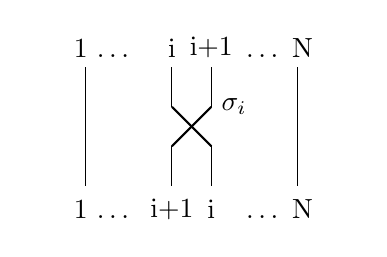
\begin{tikzpicture}
        % Draw vertical lines
        \foreach \x/\label in {1/~~~~1~\ldots, 2.1/i, 2.6/i+1, 3.7/\ldots~N~~~~~} {
            \draw (\x,0) -- (\x,1.5) node[above] {\label};
        }
    
        % Exchange between the i and j lines
        \draw[thick, white] (2.1,0.5) -- (2.1,1);
        \draw[thick, white] (2.6,0.5) -- (2.6,1);
        \draw[thick, black] (2.1,0.5) -- (2.6,1) node[right] {$\sigma_i$} ;
        \draw[thick, black] (2.6,0.5) -- (2.1,1);
    
        % Add numbers below the lines
        \foreach \x/\label in {1/~~~~1~\ldots, 2.1/i+1, 2.6/i, 3.7/\ldots~N~~~~~} {
            \node at (\x,-0.3) {\label};
        }
    
        \end{tikzpicture}
        \caption{A pictorial diagram of a transposition $\sigma_i$.}
        \label{fig:trasp}
    \end{figure}
    
    \begin{figure}[h]
        \centering
        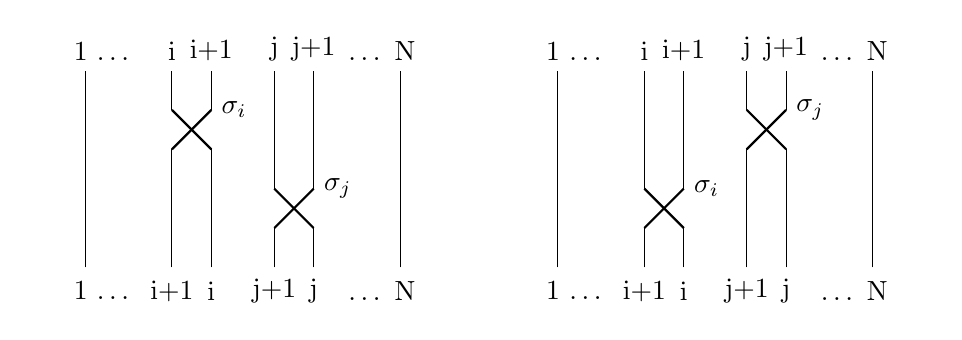
\begin{tikzpicture}
        % Draw vertical lines
        \foreach \x/\label in {1/~~~~1~\ldots, 2.1/i, 2.6/i+1, 3.4/j, 3.9/j+1, 5/\ldots~N~~~~~} {
            \draw (\x,0) -- (\x,2.5) node[above] {\label};
        }
    
        \foreach \x/\label in {7/~~~~1~\ldots, 8.1/i, 8.6/i+1, 9.4/j, 9.9/j+1, 11/\ldots~N~~~~~} {
            \draw (\x,0) -- (\x,2.5) node[above] {\label};
        }
    
        
        % Exchange between the i and j lines
        \draw[thick, white] (2.1,1.5) -- (2.1,2);
        \draw[thick, white] (2.6,1.5) -- (2.6,2);
        \draw[thick, black] (2.1,1.5) -- (2.6,2) node[right] {$\sigma_i$} ;
        \draw[thick, black] (2.6,1.5) -- (2.1,2);
        \draw[thick, white] (3.4,0.5) -- (3.4,1);
        \draw[thick, white] (3.9,0.5) -- (3.9,1);
        \draw[thick, black] (3.4,0.5) -- (3.9,1) node[right] {$\sigma_j$};
        \draw[thick, black] (3.9,0.5) -- (3.4,1);
    
        \draw[thick, white] (8.1,0.5) -- (8.1,1);
        \draw[thick, white] (8.6,0.5) -- (8.6,1);
        \draw[thick, black] (8.1,0.5) -- (8.6,1) node[right] {$\sigma_i$} ;
        \draw[thick, black] (8.6,0.5) -- (8.1,1);
        \draw[thick, white] (9.4,1.5) -- (9.4,2);
        \draw[thick, white] (9.9,1.5) -- (9.9,2);
        \draw[thick, black] (9.4,1.5) -- (9.9,2) node[right] {$\sigma_j$} ;
        \draw[thick, black] (9.9,1.5) -- (9.4,2);
        
        % Add numbers below the lines
        \foreach \x/\label in {1/~~~~1~\ldots, 2.1/i+1, 2.6/i, 3.4/j+1, 3.9/j, 5/\ldots~N~~~~~} {
            \node at (\x,-0.3) {\label};
        }
    
        \foreach \x/\label in {7/~~~~1~\ldots, 8.1/i+1, 8.6/i, 9.4/j+1, 9.9/j, 11/\ldots~N~~~~~} {
            \node at (\x,-0.3) {\label};
        }
        \end{tikzpicture}
        \caption{A pictorial diagram of a transposition $\sigma_i \sigma_j$ on the left and $\sigma_j \sigma_i$ on the right, where $|i - j| > 2$.}
        \label{fig:traspij}
    \end{figure}
    
    \begin{figure}[h]
        \centering
        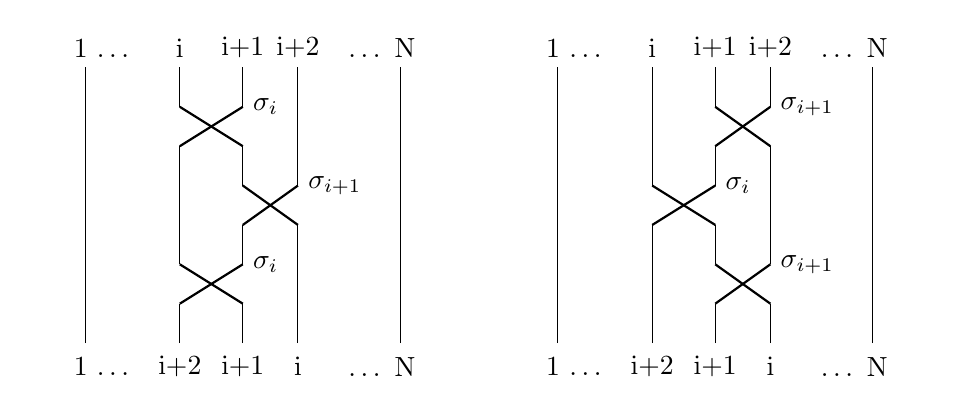
\begin{tikzpicture}
        % Draw vertical lines
        \foreach \x/\label in {1/~~~~1~\ldots, 2.2/i, 3/i+1, 3.7/i+2, 5/\ldots~N~~~~~} {
            \draw (\x,0) -- (\x,3.5) node[above] {\label};
        }
    
        \foreach \x/\label in {7/~~~~1~\ldots, 8.2/i, 9/i+1, 9.7/i+2, 11/\ldots~N~~~~~} {
            \draw (\x,0) -- (\x,3.5) node[above] {\label};
        }
    
        
        % Exchange between the i and j lines
        \draw[thick, white] (2.2,2.5) -- (2.2,3);
        \draw[thick, white] (3,2.5) -- (3,3);
        \draw[thick, black] (2.2,2.5) -- (3,3) node[right] {$\sigma_i$} ;
        \draw[thick, black] (3,2.5) -- (2.2,3);
        \draw[thick, white] (3,1.5) -- (3,2);
        \draw[thick, white] (3.7,1.5) -- (3.7,2);
        \draw[thick, black] (3,1.5) -- (3.7,2) node[right] {$\sigma_{i+1}$};
        \draw[thick, black] (3.7,1.5) -- (3,2);
        \draw[thick, white] (2.2,0.5) -- (2.2,1);
        \draw[thick, white] (3,0.5) -- (3,1);
        \draw[thick, black] (2.2,0.5) -- (3,1) node[right] {$\sigma_i$} ;
        \draw[thick, black] (3,0.5) -- (2.2,1);
    
        \draw[thick, white] (8.2,1.5) -- (8.2,2);
        \draw[thick, white] (9,1.5) -- (9,2);
        \draw[thick, black] (8.2,1.5) -- (9,2) node[right] {$\sigma_i$} ;
        \draw[thick, black] (9,1.5) -- (8.2,2);
        \draw[thick, white] (9,0.5) -- (9,1);
        \draw[thick, white] (9.7,0.5) -- (9.7,1);
        \draw[thick, black] (9,0.5) -- (9.7,1) node[right] {$\sigma_{i+1}$};
        \draw[thick, black] (9.7,0.5) -- (9,1);
        \draw[thick, white] (9,2.5) -- (9,3);
        \draw[thick, white] (9.7,2.5) -- (9.7,3);
        \draw[thick, black] (9,2.5) -- (9.7,3) node[right] {$\sigma_{i+1}$};
        \draw[thick, black] (9.7,2.5) -- (9,3);
        
        
        % Add numbers below the lines
        \foreach \x/\label in {1/~~~~1~\ldots, 2.2/i+2, 3/i+1, 3.7/i, 5/\ldots~N~~~~~} {
            \node at (\x,-0.3) {\label};
        }
    
        \foreach \x/\label in {7/~~~~1~\ldots, 8.2/i+2, 9/i+1, 9.7/i, 11/\ldots~N~~~~~} {
            \node at (\x,-0.3) {\label};
        }
        \end{tikzpicture}
        \caption{A pictorial diagram of a transposition $\sigma_i \sigma_{i+1} \sigma_i$ on the left and $\sigma_{i+1} \sigma_i \sigma_{i+1}$ on the right.}
        \label{fig:traspi1}
    \end{figure}

    \begin{figure}[h]
        \centering
        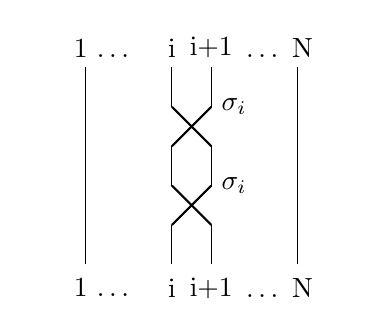
\begin{tikzpicture}
        % Draw vertical lines
        \foreach \x/\label in {1/~~~~1~\ldots, 2.1/i, 2.6/i+1, 3.7/\ldots~N~~~~~} {
            \draw (\x,0) -- (\x,2.5) node[above] {\label};
        }
    
        
        % Exchange between the i and j lines
        \draw[thick, white] (2.1,0.5) -- (2.1,1);
        \draw[thick, white] (2.6,0.5) -- (2.6,1);
        \draw[thick, black] (2.1,0.5) -- (2.6,1) node[right] {$\sigma_i$} ;
        \draw[thick, black] (2.6,0.5) -- (2.1,1);
    
        \draw[thick, white] (2.1,1.5) -- (2.1,2);
        \draw[thick, white] (2.6,1.5) -- (2.6,2);
        \draw[thick, black] (2.1,1.5) -- (2.6,2) node[right] {$\sigma_i$} ;
        \draw[thick, black] (2.6,1.5) -- (2.1,2);
    
        
        % Add numbers below the lines
        \foreach \x/\label in {1/~~~~1~\ldots, 2.1/i, 2.6/i+1, 3.7/\ldots~N~~~~~} {
            \node at (\x,-0.3) {\label};
        }
    
        \end{tikzpicture}
        \caption{A pictorial diagram of a transposition $(\sigma_i)^2$.}
        \label{fig:trasp2}
    \end{figure}

\section{Bosons and fermions}

    Now, we are able to calculate explicitly~\eqref{perm:phase}, which is 
    \begin{equation}
        \alpha_P = \alpha_1 + \ldots \alpha_N~,
    \end{equation}
    where $\alpha_i$ is the phase factor that label the transposition $\sigma_{\alpha_i}$, i.e.
    \begin{equation*}
        \psi(\sigma_{\alpha_i}(x_1,\ldots x_N)) = \exp(i \alpha_i) \psi (x_1,\ldots x_N) ~.
    \end{equation*}
    \begin{proof}
        In fact, using~\eqref{perm:dec} and properties of the exponential, we obtain
        \begin{equation*}
        \begin{aligned}
            \psi(P(x_1,\ldots, x_N)) & = \psi((\sigma_{\alpha_1} \ldots \sigma_{\alpha_N}) (x_1,\ldots, x_N)) \\ & = \exp (i \alpha_1) \psi((\sigma_{\alpha_2} \ldots \sigma_{\alpha_N}) (x_1,\ldots, x_N)) \\ & ~~ \vdots \\ & = \exp (i \alpha_1) \ldots \exp (i \alpha_N) \psi(x_1,\ldots, x_N) \\ & = \exp (i \underbrace{(\alpha_1 + \ldots \alpha_N)}_{\alpha_P}) \psi(x_1,\ldots x_N) \\ &  = \exp (i \alpha_P) \psi(x_1,\ldots, x_N) ~.
        \end{aligned}
        \end{equation*}
    \end{proof}
    Furthermore, we can also find which are the possible values of $\alpha_P$:
    \begin{enumerate}
        \item $\alpha_P = 0$ and $\exp(i \alpha_P) = 1$, which correspond respectively to a bosonic totally symmetric wavefunction, i.e.~under $P$
        \begin{equation*}
            \psi(x_1, \ldots x_N) \xmapsto{P} (+ 1) \psi(x_1, \ldots x_N) ~,
        \end{equation*}
        \item $\alpha_P = \pi$ and $\exp(i \alpha_P) = \sgn(P)$, which correspond respectively to a fermionic totally antysymmetric wavefunction, i.e.~under $P$
        \begin{equation*}
            \psi(x_1, \ldots x_N) \xmapsto{P} \sgn(P) \psi(x_1, \ldots x_N) = \begin{cases}
                + \psi(x_1, \ldots x_N) & \sgn(P) = +1 \\
                - \psi(x_1, \ldots x_N) & \sgn(P) = - 1 \\
            \end{cases} ~.
        \end{equation*}
    \end{enumerate}
    Coming to hand a theorem that can be proved only in the realm of quantum field theory,  the spin-statistic theorem, we can associate a particular value of the spin to this two statistics: bosons, which have symmetric wavefunctions, are associated to integer spin particles, whereas fermions, which have antisymmetric wavefunctions, are associated to half-integer spin particles.
    \begin{proof}
        Using~\eqref{perm:1}
        \begin{equation*}
            \psi(x_1, \ldots x_N) \xmapsto{\sigma_i} \exp(i \alpha_i) \psi(x_1, \ldots x_N)\xmapsto{\sigma_i \sigma_j} \exp(i \alpha_i) \exp(i \alpha_j) \psi(x_1, \ldots x_N) ~,
        \end{equation*}
        \begin{equation*}
            \psi(x_1, \ldots x_N) \xmapsto{\sigma_j} \exp(i \alpha_j) \psi(x_1, \ldots x_N)\xmapsto{\sigma_j \sigma_i} \exp(i \alpha_j) \exp(i \alpha_i) \psi(x_1, \ldots x_N) ~,
        \end{equation*}
        hence 
        \begin{equation*}
            \exp(i \alpha_i) \exp(i \alpha_j) = \exp(i \alpha_j) \exp(i \alpha_i) ~,
        \end{equation*}
        which means that they commute
        \begin{equation}\label{pr1}
            \alpha_i + \alpha_j = \alpha_j +\alpha_i ~.
        \end{equation}
        Using~\eqref{perm:2}
        \begin{equation*}
        \begin{aligned}
            \psi(x_1, \ldots x_N) & \xmapsto{\sigma_i} \exp(i \alpha_i) \psi(x_1, \ldots x_N) \\ & \xmapsto{\sigma_i \sigma_{i+1}} \exp(i \alpha_i) \exp(i \alpha_{i+1}) \psi(x_1, \ldots x_N) \\ & \xmapsto{\sigma_i \sigma_{i+1} \sigma_i} \exp(i \alpha_i) \exp(i \alpha_{i+1}) \exp(i \alpha_i) \psi(x_1, \ldots x_N) ~,
        \end{aligned}
        \end{equation*}
        \begin{equation*}
        \begin{aligned}
            \psi(x_1, \ldots x_N) & \xmapsto{\sigma_{i+1}} \exp(i \alpha_{i+1}) \psi(x_1, \ldots x_N) \\ & \xmapsto{\sigma_{i+1} \sigma_i} \exp(i \alpha_{i+1}) \exp(i \alpha_i) \psi(x_1, \ldots x_N) \\ & \xmapsto{\sigma_{i+1} \sigma_i \sigma_{i+1} } \exp(i \alpha_{i+1}) \exp(i \alpha_i) \exp(i \alpha_{i+1}) \psi(x_1, \ldots x_N) ~,
        \end{aligned}
        \end{equation*}
        hence 
        \begin{equation*}
            \exp(i \alpha_i) \exp(i \alpha_{i+1}) \exp(i \alpha_i) = \exp(i \alpha_{i+1}) \exp(i \alpha_i) \exp(i \alpha_{i+1}) ~,
        \end{equation*}
        which means that 
        \begin{equation}\label{pr2}
           \alpha_i + \alpha_{i+1} + \alpha_i = \alpha_{i+1} + \alpha_i + \alpha_{i+1} ~. 
        \end{equation}
        Putting together this two properties~\eqref{pr1} and ~\eqref{pr2}, we have
        \begin{equation*}
            \alpha_i + \alpha_{i+1} + \alpha_i = \alpha_{i+1} + \alpha_i + \alpha_{i+1} ~,
        \end{equation*}
        \begin{equation*}
            \cancel{\alpha_{i+1}} + \cancel{\alpha_i }+ \alpha_i = \cancel{\alpha_{i+1}} + \cancel{\alpha_i} + \alpha_{i+1} ~,
        \end{equation*}
        \begin{equation*}
            \alpha_i = \alpha_{i+1} ~.
        \end{equation*}
        Therefore, $\forall i= 1, \ldots N-1$ and $\alpha_i \in [0, 2\pi[$ we have $\alpha_i = \alpha_{i+1} = \alpha$.
        Using~\eqref{prop3}
        \begin{equation*}
            \exp(i \alpha)^2 = \exp (2 i \alpha) = \mathbb I = \exp(0) ~,
        \end{equation*}
        which means that 
        \begin{equation*}
            \alpha = 0, \pi ~.
        \end{equation*}
        Finally, there are only two possibilities 
        \begin{equation*}
            \psi(x_1, \ldots x_N) \xmapsto{\sigma_i} \underbrace{\exp(i 0)}_{+1} \psi(x_1, \ldots x_N) = \psi(x_1, \ldots x_N)
        \end{equation*}
        and 
        \begin{equation*}
            \psi(x_1, \ldots x_N) \xmapsto{\sigma_i} \underbrace{\exp(i \pi)}_{-1} \psi(x_1, \ldots x_N) = - \psi(x_1, \ldots x_N)~.
        \end{equation*}
    \end{proof}

\chapter{Second quantisation}

    The Hilbert space of indistinguishable particle is smaller than the distinguishable one, because we have seen that the phase factor can only have two possible values. In this chapter, we will see how we can describe such spaces, in terms of the symmetrised or antisymmetrised Hilbert space $\mathcal H_{S/A}$ in the language of first quantisation and in terms of the Fock space $\mathcal F_{B/F}$ in the language of second quantisation.

\section{Symmetric/antisymmetric Hilbert space} 

    Consider $2$ particles. If they are distinguishable, the total Hilbert space is 
    \begin{equation*}
        \mathcal H_{tot} = \mathcal H \otimes \mathcal H ~,
    \end{equation*}
    whereas if the particles are indistinguishable, we can decompose the Hilbert space into
    \begin{equation*}
        \mathcal H_{tot} = \mathcal H_S \oplus_\perp  \mathcal H_A ~.
    \end{equation*} 
    \begin{proof}
        In fact, given two states $\ket{a}_1 \in \mathcal H_1$ and $\ket{b}_2 \in \mathcal H_2$, we have 
    \begin{equation*}
    \begin{aligned}
        \ket{a}_1\ket{b}_2 & = \frac{2}{2} \ket{a}_1\ket{b}_2 + \frac{1}{2} \ket{b}_1\ket{a}_2 - \frac{1}{2} \ket{b}_1\ket{a}_2 \\ & = \underbrace{\frac{\ket{a}_1\ket{b}_2 + \ket{b}_1\ket{a}_2}{2}}_{\ket{\psi_S}} + \underbrace{\frac{\ket{a}_1\ket{b}_2 - \ket{b}_1\ket{a}_2}{2}}_{\ket{\psi_A}} \\ & = \ket{\psi_S} + \ket{\psi_A} ~.
    \end{aligned}
    \end{equation*}
    Furthermore, the permutation group for $2$ particles is $P_2 = \{\mathbb I, \sigma\}$. The symmetric part $\ket{\psi_S} \in \mathcal H_S$, since
    \begin{equation*}
        \sigma \ket{\psi_S} = \sigma \frac{\ket{a}_1\ket{b}_2 + \ket{b}_1\ket{a}_2}{2} = \frac{\ket{b}_1\ket{a}_2 + \ket{a}_1\ket{b}_2}{2} = \frac{\ket{a}_1\ket{b}_2 + \ket{b}_1\ket{a}_2}{2} = \ket{\psi_S} ~,
    \end{equation*}
    where we used the commutativity property. The antisymmetric part is $\ket{\psi_A} \in \mathcal H_A$, since
    \begin{equation*}
        \sigma \ket{\psi_A} = \sigma \frac{\ket{a}_1\ket{b}_2 - \ket{b}_1\ket{a}_2}{2} = \frac{\ket{b}_1\ket{a}_2 - \ket{a}_1\ket{b}_2}{2} = - \frac{\ket{a}_1\ket{b}_2 - \ket{b}_1\ket{a}_2}{2} = - \ket{\psi_A} ~,
    \end{equation*}
    where we used the commutativity property. Finally, the decomposition is orthogonal, since 
    \begin{equation*}
    \begin{aligned}
        \braket{\psi_S}{\psi_A} & = \frac{\bra{a}_1\bra{b}_2 + \bra{b}_1\bra{a}_2}{2} \frac{\ket{a}_1 \ket{b}_2 - \ket{b}_1 \ket{a}_2}{2} \\ & = \frac{1}{4} (\underbrace{\braket{a}{a}_1}_1 \underbrace{\braket{b}{b}_2}_1 - \braket{a}{b}_1 \braket{b}{a}_2 + \braket{b}{a}_1 \braket{a}{b}_2 - \underbrace{\braket{b}{b}_1}_1 \underbrace{\braket{a}{a}_2}_1) \\ & = \frac{1}{4} (- \braket{a}{b}_1 \braket{b}{a}_2 + \braket{b}{a}_1 \braket{a}{b}_2)  
    \end{aligned}
    \end{equation*}
    and 
    \begin{equation*}
    \begin{aligned}
        - \braket{\psi_S}{\psi_A} & = - \frac{\bra{a}_1\bra{b}_2 + \bra{b}_1\bra{a}_2}{2} \frac{\ket{a}_1 \ket{b}_2 - \ket{b}_1 \ket{a}_2}{2} \\ & = - \frac{1}{4} (\underbrace{\braket{a}{a}_1}_1 \underbrace{\braket{b}{b}_2}_1 - \braket{a}{b}_1 \braket{b}{a}_2 + \braket{b}{a}_1 \braket{a}{b}_2 - \underbrace{\braket{b}{b}_1}_1 \underbrace{\braket{a}{a}_2}_1) \\ & = - \frac{1}{4} (- \braket{a}{b}_1 \braket{b}{a}_2 + \braket{b}{a}_1 \braket{a}{b}_2) \\ & = \frac{1}{4} (- \braket{a}{b}_2 \braket{b}{a}_1 + \braket{b}{a}_2 \braket{a}{b}_1 ) ~,
    \end{aligned}
    \end{equation*}
    which means that $\braket{\psi_S}{\psi_A} = - \braket{\psi_S}{\psi_A}$. Therefore, the only solution is $\braket{\psi_S}{\psi_A} = 0$.
    \end{proof}
    
    Notice that Pauli's exclusion principle is encoded into the antisymmetric part, because if $a = b$ we have $\ket{\psi_A} = 0$.

    This decomposition is equivalent to define two orthogonal projectors: the symmetriser 
    \begin{equation*}
        \hat S \colon \mathcal H \rightarrow \mathcal H_S
    \end{equation*}
    and the antisymmetriser 
    \begin{equation*}
        \hat A \colon \mathcal H \rightarrow \mathcal H_A ~,
    \end{equation*}
    such that they satisfy the properties 
    \begin{equation}\label{projprop}
        \hat S^\dagger = \hat S~, \quad \hat A^\dagger = \hat A~, \quad \hat S^2 = \hat S~, \quad \hat A^2 = \hat A~, \quad \hat S \hat A = \hat A \hat S = 0 ~.
    \end{equation}

    Generalising for $N$ particles, if they are distinguishable, the total Hilbert space is 
    \begin{equation*}
        \mathcal H_{tot} = \mathcal H \otimes \ldots \mathcal H
    \end{equation*}
    and a state is $\ket{\psi} = \ket{a_1}_1 \ldots \ket{a_N}_N = \ket{1, \ldots N}$ where $\ket{a_j} \in \mathcal H$. 
    However, if the particle are indistinguishable, similarly to before, we can define the symmetriser
    \begin{equation*}
        \hat S \colon \ket{\psi} \mapsto \frac{1}{N!} \sum_{P \in P_N} \hat P \ket{1, \ldots, N} = \frac{1}{N!} \sum_{P \in P_N} \ket{P(1), \ldots, P(N)}
    \end{equation*}
    and the antisymmetriser
    \begin{equation*}
        \hat A \colon \ket{\psi} \mapsto \frac{1}{N!} \sum_{P \in P_N} sgn(P) \hat P \ket{1, \ldots, N} = \frac{1}{N!} \sum_{P \in P_N} sgn(P) \ket{P(1), \ldots, P(N)} ~,
    \end{equation*}
    where $\hat P: (1, \ldots N) \mapsto (P(1), \ldots P(N))$. Intuitively, this means that we have to permute all the possible indices $1, \ldots N$, keeping in mind the parity if we use the antisymmetriser. They satisfy the orthogonal projector properties~\eqref{projprop}. Notice that for $N > 2$ particles, the total Hilbert space is $\mathcal H_{tot} = \mathcal H_S \otimes \mathcal H_A \otimes \mathcal H'$, where bosons work only in $\mathcal H_S$, fermions work only in $\mathcal H_A$ and $\mathcal H'$ is not physical.

    \begin{example}
        For $N=3$, we can have $\psi_S \in \mathcal H_S$
        \begin{equation*}
            \psi_S = \hat S \psi = \psi(1,2,3) + \psi(1,3,2) + \psi(2,1,3) + \psi(2,3,1) + \psi(3,1,2) + \psi(3,2,1)
        \end{equation*}
        and $\psi_A \in \mathcal H_A$
        \begin{equation*}
            \psi_A = \hat A \psi = \psi(1,2,3) - \psi(1,3,2) - \psi(2,1,3) + \psi(2,3,1) + \psi(3,1,2) - \psi(3,2,1) ~.
        \end{equation*}
        However, we can also have $\psi' \in \mathcal H'$ such that
        \begin{equation*}
            \psi' = \psi(1,2,3) + \psi(1,3,2) -  \psi(2,1,3) - \psi(2,3,1) + \psi(3,1,2) + \psi(3,2,1) ~.
        \end{equation*}
    \end{example}
    
    For $N$ distinguishable particle, consider an orthonormal basis for the total Hilbert space
    \begin{equation*}
        \{u_{\alpha_1}(x_1) \ldots u_{\alpha_N}(x_N)\}_{\alpha_1, \ldots \alpha_N=0}^\infty ~,
    \end{equation*}
    where $\{u_{\alpha_K} (x_k)\}_{\alpha_k = 1}^\infty$ is an orthonormal basis for a single Hilbert space $\mathcal H_1$. Notice that they are labelled by the ordered set $(\alpha_1, \ldots \alpha_N)$ and we are specifying which particle is in which states. 
    On the orher hand, in order to construct an orthonormal basis for $\mathcal H_A$ and $\mathcal H_S$ for $N$ indistinguishable particles, we project the distinguishable orthonormal basis respectively with the antisymmetriser and the symmetriser
    \begin{equation}\label{onbas}
        \ket{n_1, \ldots n_j, \ldots} = C \begin{cases} \hat S \\ \hat A \end{cases} ~ u_{\alpha_1}(x_1) \ldots u_{\alpha_N}(x_N) ~,
    \end{equation}
    where $C$ is a normalisation constant. In fact, bb the properties of the projectors, they are orthonormal but they are not normalised. Therefore, we need to choose a normalisation constant
    \begin{equation*}
        C = \begin{cases}
            \sqrt{\frac{N!}{n_1! \ldots n_k! \ldots}} & \text{for}~ \mathcal H_S \\
            \sqrt{N!} & \text{for}~ \mathcal H_A \\
        \end{cases} ~.
    \end{equation*}
    On the contrary with respect to the distinguishable case, now we lose information, since we know only how many particles are in each state and not anymore which is in which state. In fact, we label the states with $n_1, \ldots n_k, \dots$ with $j=1, \ldots \infty$, which are the occupation number. For bosons, we have $n_k = 0, 1, \ldots, \infty$, whereas for fermions, we have $n_k = 0, 1$. For both cases, there is the constraint $N = \sum_k n_k$, which is an infinite sum but mostly are zero occupied. Moreover, given the set $\alpha_k$, we uniquely determine the occupation number $n_k$. On the other hand, given the occupation number $n_k$, we use the symmetric or antisymmetric properties~\eqref{onbas} to uniquely determine the state, because it is in $1-1$ correspondence to the set $n_k$. This means that we can describe the system using a different approch, based on the occupation number rathen than what we have done so far, called second quantisation, because we make a further quantisation by promoting fields to operators.

\section{Bosonic and fermionic ladder operators}

    In order to construct the Fock space, we need operators to move from an Hilbert space to another with different number of particles. By analogy with the harmonic oscillator, we introduce the ladder operators. 

    The bosonic creation and annihilation operators are the one such that they satisfy the following properties 
    \begin{equation}\label{bos}
        [\hat a, \hat a^\dagger]_- = \hat a \hat a^\dagger - \hat a^\dagger \hat a = \mathbb I~.
    \end{equation}
    Furthermore, the number operator $\hat N = \hat a^\dagger \hat a$ such that 
    \begin{equation*}
        [\hat N, \hat a] = - \hat a~, \quad [\hat N, \hat a^\dagger] = \hat a^\dagger ~.
    \end{equation*} 
    The ground state (vacuum) is 
    \begin{equation*}
        \hat a \ket{0} = 0
    \end{equation*}
    and a generic state is defined by
    \begin{equation*}
        \ket{\psi} = \frac{1}{\sqrt{n!}} (\hat a^\dagger)^n \ket{0} ~.
    \end{equation*}

    The fermionic creation and annihilation operators are the one such that they satisfy the following properties 
    \begin{equation}\label{ferm}
        [\hat a, \hat a^\dagger]_+ = \hat a \hat a^\dagger + \hat a^\dagger \hat a = \mathbb I ~.
    \end{equation}
    Furthermore, the number operator $\hat N = \hat a^\dagger \hat a$ such that 
    \begin{equation*}
        [\hat N, \hat a] = - \hat a~, \quad [\hat N, \hat a^\dagger] = \hat a^\dagger ~.
    \end{equation*} 
    The ground state (vacuum) is
    \begin{equation*}
        \hat a \ket{0} = 0 ~,
    \end{equation*}
    and a generic state is defined by
    \begin{equation*}
        \ket{\psi} = \frac{1}{\sqrt{n!}} (\hat a^\dagger)^N \ket{0} ~.
    \end{equation*}
    However, the anticommutator relation ensures the validity of the Pauli's exclusion principle. In fact, we have 
    \begin{equation*}
        \hat a^2 = (\hat a^\dagger)^2 = 0 ~.
    \end{equation*}

\section{Fock space}

    Now, we need to build the Fock space. 
    
    First, consider a single particle Hilbert space $\mathcal H$ with an orthonormal basis $\{\ket{e_k}\}_{n=1}^\infty$. To each $\ket{e_k}$, we associate annihilation and creation operators
    \begin{equation*}
        \ket{e_k} \mapsto \{\hat a_k, \hat a_k^\dagger\} ~,
    \end{equation*}
    such that they satisfy
    \begin{equation}\label{comm}
        [\hat a_k, \hat a_j]_\pm = [\hat a_k^\dagger, \hat a_j^\dagger]_\pm = 0 ~, \quad [\hat a_k, \hat a_j^\dagger]_\pm = \delta_{kj} ~,
    \end{equation}
    where the minus sign corresponds to the commutator (bosons)~\eqref{bos} and the plus sign to the anticommutator (fermions)~\eqref{ferm}. The normalised vacuum state is defined by the annihilation of every annihilation operator
    \begin{equation*}
        \hat a_k \ket{0} = 0 \quad \forall n~.
    \end{equation*}
    It generates a subspace of dimension $1$ 
    \begin{equation}\label{vac}
        \mathcal H^{(0)}_{S/A} = \{\lambda \ket{0} \colon \lambda \in \mathbb C \} ~.
    \end{equation}
    For each $\ket{e_k}$, we can also associate a number operator $\hat n_k = \hat a_k^\dagger \hat a_k$ such that 
    \begin{equation*}
        \hat n_k \hat a_k^\dagger \ket{0} = 1 \hat a_k^\dagger \ket{0} ~, \quad \hat n_{k'} \hat a_k \ket{0} = 0 \quad k' \neq k ~.
    \end{equation*}

    By analogy, we can define the $1$-particle state
    \begin{equation*}
        \ket{0, \ldots, 1_k, \ldots, 0} = \hat a_k^\dagger \ket{0, \ldots, 0} ~,
    \end{equation*}
    where explicitly means that $\ket{n_1=0, \ldots, n_k=1, \ldots}$. Continuing with this process, we can construct the whole Fock space. Notice, however, that even when we have only $2$ states, bosons and fermions behave differently. In fact, for
    \begin{equation*}
        \hat a_{k_1}^\dagger \hat a_{k_2}^\dagger \ket{0} = \ket{e_{k_1}} \ket{e_{k_2}} 
    \end{equation*}
    we have for fermions, if $k_1 = k_2 = k$
    \begin{equation*}
    (\hat a^\dagger_k)^2 \ket{0} = 0 ~,
    \end{equation*}
    whereas for bosons 
    \begin{equation*}
        (\hat a^\dagger_k)^2 \ket{0} \neq 0 ~.
    \end{equation*}
    Furthermore, if $k_1 \neq  k_2$, we have for fermions
    \begin{equation*}
        \hat a^\dagger_{k_1} \hat a^\dagger_{k_2} \ket{0} = - \hat a^\dagger_{k_2} \hat a^\dagger_{k_1} \ket{0} ~,
    \end{equation*}
    whereas for bosons 
    \begin{equation*}
        \hat a^\dagger_{k_1} \hat a^\dagger_{k_2} \ket{0} = \hat a^\dagger_{k_2} \hat a^\dagger_{k_1} \ket{0} ~.
    \end{equation*}

    The general construction can be made, recalling that there is a $1-1$ correspondence between the orthonormal basis $\{\ket{e_n}\}_{n=1}^\infty$ of $\mathcal H$ and the orthonormal basis $\{\hat a_k \ket{0}\}_{k=1}^\infty$ of $\mathcal H_{S/A}$. Hence, for $N$ particles, we define
    \begin{equation*}
        \mathcal H_{S/A}^{(N)} = \{\ket{n_1, \ldots n_k, \ldots} = \frac{1}{\sqrt{ \prod_j n_j}} (\hat a_1^\dagger)^{n_1} \ldots (\hat a_k^\dagger)^{n_k} \ldots \ket{0} \} ~.
    \end{equation*} 
    If $N$ is not fixed, like the passage from canonical to grand canonical ensemble, the total Fock space is 
    \begin{equation*}
        \mathcal F = \bigoplus_{N=0}^\infty \mathcal H^{(N)}_{S/A} ~.
    \end{equation*} 
    It satisfies the following properties 
    \begin{enumerate}
        \item orthonormality, i.e. 
            \begin{equation*}
                \braket{{n'}_1, \ldots {n'}_k, \ldots}{n_1, \ldots n_k, \ldots} = \delta_{{n'}_1, n_1} \ldots \delta_{{n'}_k, n_k} \ldots  ~,
            \end{equation*}
        \item annihilation $\hat a_k \colon \mathcal H^{(N)}_{S/A} \rightarrow \mathcal H^{(N-1)}_{S/A}$, i.e.
            \begin{equation*}
                \hat a_k \ket{n_1, \ldots n_k, \ldots} = \eta_k \sqrt{n_k} \ket{n_1, \ldots (n_k - 1), \ldots} ~,
            \end{equation*}
            where for bosons $\eta_k = 1$ and for fermions $\eta_k = (-1)^{\sum_{j < k} n_j}$,
        \item creation $\hat a_k^\dagger \colon \mathcal H^{(N)}_{S/A} \rightarrow \mathcal H^{(N+1)}_{S/A}$, i.e. for bosons
            \begin{equation*}
                \hat a^\dagger_k \ket{n_1, \ldots n_k, \ldots} = \sqrt{n_k + 1} \ket{n_1, \ldots (n_k + 1), \ldots} ~,
            \end{equation*}
            and for fermions
            \begin{equation*}
                \hat a^\dagger_k \ket{n_1, \ldots n_k, \ldots} = \eta_k \sqrt{1 - n_k} \ket{n_1, \ldots (n_k + 1), \ldots} ~,
            \end{equation*}
        \item number operator $\hat n_k = \hat a_k^\dagger \hat a_k$ such that 
            \begin{equation*}
                \hat n_k \ket{n_1, \ldots n_k, \ldots} = n_k \ket{n_1, \ldots n_k, \ldots}
            \end{equation*}
        and the total number operator $\hat N = \sum_k \hat n_k = \sum_k \hat a^\dagger_k \hat a_k$ such that 
        \begin{equation*}
            \hat N \ket{n_1, \ldots n_k, \ldots} = \Big (\sum_k n_k \Big ) \ket{n_1, \ldots n_k, \ldots} ~.
        \end{equation*}
    \end{enumerate}

\section{Field operators} 

    Having constructed the Fock space, now we are looking for observables, i.e.~operators. 
    Consider a generic particle state, given by the wavefunction $\ket{f} \in \mathcal H$. We can expand it into the basis $\{\ket{e_k}\}$, using the completeness relation, to find 
    \begin{equation*}
        \ket{f} = \ket{f} \mathbb I = \sum_k \braket{e_k}{f} \ket{e_k} = \sum_k f_k \ket{e_k}
    \end{equation*}
    which by the previous construction, is equivalent to 
    \begin{equation}\label{op1}
        \ket{f} = \sum_k f_k \hat a_k^\dagger \ket{0}
    \end{equation}
    Therefore, it is natural to define also operators expanded in the basis of the ladder operators
    \begin{equation}\label{op2}
        \hat \psi^\dagger (f) = \sum_k f_k \hat a^\dagger_k ~, \quad \hat \psi (f) = \sum_k f_k^* \hat a_k ~,
    \end{equation}
    in order to get a state $\hat \psi (f) \ket{0}$. 
    \begin{proof}
        In fact, combining~\eqref{op1} and~\eqref{op2}, we have
        \begin{equation*}
            \ket{f} = \underbrace{\sum_k f_k \hat a_k^\dagger}_{\hat \psi(f)} \ket{0} = \hat \psi (f) \ket{0} ~.
        \end{equation*}
    \end{proof}
    The related commutator relations of the operators can be written in terms of the braket product of states as
    \begin{equation}\label{commf}
        [\hat \psi (f), \hat \psi^\dagger (g)]_\pm = \braket{f}{g}\mathbb I ~.
    \end{equation}
    \begin{proof}
        In fact, using~\eqref{comm}
        \begin{equation*}
        \begin{aligned}
            [\hat \psi (f), \hat \psi^\dagger (g)]_\pm & = [\sum_k f^*_k \hat a_k, \sum_m g_m \hat a^\dagger]_\pm = \sum_k \sum_m f^*_k g_m \underbrace{[\hat a_k, \hat a^\dagger_m]}_{\delta_{km} \mathbb I} \\ & = \sum_k f^*_k g_k \mathbb I = \braket{f}{g} \mathbb I ~,
        \end{aligned}
        \end{equation*}
        where we have used 
        \begin{equation*}
            \ket{f} = \sum_k f_k \ket{e_k} ~, \quad \ket{g} = \sum_m g_m \ket{e_m} ~, \quad \braket{f}{g} = \sum_k \sum_m f^*_k g_m \underbrace{\braket{e_k}{e_m}}_{\delta_{km}} = \sum_k f^*_k g_k ~.
        \end{equation*}
    \end{proof}
    
    Now, we switch into the coordinate representation. Consider a single particle state in $\mathcal H = L^2(\mathbb R^d) \ni \psi(x)$ with an orthonormal basis $u_k(x)$ such that to each ket there are ladder operators $\hat a_k$ and $\hat a_k^\dagger$. Hence, $L^2(\mathbb R^d) \ni f(x) = \sum_k f_k u_k(x)$ and we define field operators
    \begin{equation*}
        \hat \psi(x) = \sum_k u_k (x) \hat a_k ~, \quad \hat \psi^\dagger (x) = \sum_k u_k^* (x) \hat a_k^\dagger ~,
    \end{equation*}
    which is a linear superposition of annihilation and creation operators. Actually, it is called an operator-valued function because its output is an operator. In fact, $\hat \psi(x)$ and $\hat \psi (f)$ are related by
    \begin{equation*}
        \hat \psi^\dagger (f) = \sum_k \hat a_k^\dagger f_k = \sum_k \hat a_k^\dagger \int_{\mathbb R^d} d^d x ~ u^*_k(x) f(x) = \int_{\mathbb R^d} d^d x ~ \psi^\dagger (x) \sum_k u_k^* (x) \hat a_k^\dagger ~,
    \end{equation*}
    where we have exchanged sum and integral because they are convergent. 
    The commutation relation becomes
    \begin{equation*}
        [\hat \psi(x), \hat \psi^\dagger (y)] = \delta (x - y)  \mathbb I ~.
    \end{equation*}
    \begin{proof}
        In fact,
        \begin{equation*}
        \begin{aligned}
            [\hat \psi (f), \hat \psi^\dagger (g)]_\pm & = [\int d^d x ~ f^* (x) \hat \psi(x), \int d^d y ~ g(y) \hat \psi^\dagger (y)]_\pm \\ & = \int d^d x \int d^d y ~ f^*(x) g(y) [\psi(x), \psi^\dagger (y)]  ~,
        \end{aligned}
        \end{equation*}
        which, by~\eqref{commf}, must be equal to 
        \begin{equation*}
            \braket{f}{g} = \int d^d x ~ f^* (x) g(x) ~.
        \end{equation*}
        Hence, the only possibility is
        \begin{equation*}
            [\psi(x), \psi^\dagger (y)] = \delta (x - y) \mathbb I ~.
        \end{equation*}
    \end{proof}

    \begin{example}
        Consider a plane wave basis $u(x) = \exp (i \mathbf k \cdot \mathbf x) $. Then we have $\hat \psi(x) = \sum_k \hat a_k^\dagger \exp(i \mathbf k \cdot \mathbf x)$.
    \end{example}

    Notice that field operators are basis independent.
    \begin{proof}
        In fact, consider a different basis $\{\ket{b_j}\}$ with ladder operators $\{ \hat c_j, \hat c_j^\dagger\}$, such that 
        \begin{equation*}
            \hat c_j = \sum_k \braket{b_j}{e_k} \hat a_k ~, \quad \hat c_j^\dagger = \sum_k \braket{e_k}{b_j} \hat a_k^\dagger ~.
        \end{equation*}
        Hence, expanding the wavefunction into the two basis 
        \begin{equation*}
            \ket{f} = \sum_k \braket{e_k}{f} e_k = \sum_j \braket{b_j}{f} b_j ~,
        \end{equation*}
        we find that $\hat \psi(f)$ and $\hat \psi^\dagger (f)$ are left unchanged 
        \begin{equation*}
        \begin{aligned}
            \hat \psi(f) & = \sum_k f_k^* \hat a_k = \sum_k \braket{f}{e_k} \hat a_k = \sum_k \sum_j \braket{f}{e_k} \ket{b_j} \bra{b_j} \hat a_k \\ & = \sum_j \braket{f}{b_j} \underbrace{\sum_k \braket{b_j}{e_k} \hat a_k}_{\hat b_j} = \sum_j \braket{f}{b_j} \hat b_j = \sum_j f^{'*}_j  \hat b_j  ~,
        \end{aligned}
        \end{equation*}
        and 
        \begin{equation*}
        \begin{aligned}
            \hat \psi^\dagger (f) & = \sum_k f_k \hat a_k^\dagger = \sum_k \braket{e_k}{f} \hat a_k^\dagger = \sum_k \sum_j \braket{e_k}{f} \ket{b_j} \bra{b_j} \hat a_k^\dagger \\ & = \sum_j \braket{b_j}{f} \underbrace{\sum_k \braket{e_k}{b_j} \hat a_k^\dagger}_{\hat b_j^\dagger} = \sum_j \braket{b_j}{f} \hat b_j^\dagger = \sum_j f'_j  \hat b_j^\dagger  ~,
        \end{aligned}
        \end{equation*}
    \end{proof}

    We define a one-body operator in the subspace $\mathcal H^{N}$ as 
    \begin{equation*}
        \hat O^{(1)} = \sum_{j=1}^{N} \hat O(\hat x_j, \hat p_j) ~,
    \end{equation*}
    where $\hat O(\hat x_j, \hat p_j)$ is an operator on $\mathcal H$. Since it is a sum of self-adjoint operators and thus itself self-adjoint, it exists an orthonormal basis of eigenvalues $\{u_\alpha (x)\}$ such that 
    \begin{equation}\label{evop}
        \hat O(\hat p, \hat x) u_\alpha (x) = \epsilon_\alpha u_\alpha (x) ~.
    \end{equation}

    In first quantisation language, given an orthonormal basis~\eqref{onbas}
    \begin{equation*}
        \psi_{n_1 \ldots n_k \ldots} (x_i, \ldots, x_k, \ldots) = C_N \begin{bmatrix}
            \hat S \\ \hat A
        \end{bmatrix} u_{\alpha_1} (x_1) \ldots u_{\alpha_k}(x_k) \ldots ~,
    \end{equation*}
    we have
    \begin{equation*}
        \hat O^{(1)} \psi_{n_1 \ldots n_k \ldots} (x_1, \ldots x_k, \ldots) = \Big (\sum_{j=1}^{\infty} \epsilon_j n_j \Big ) \psi_{n_1 \ldots n_k \ldots} (x_1, \ldots x_k, \ldots) ~.
    \end{equation*}
    \begin{proof}
    In fact, using~\eqref{evop}, we obtain
    \begin{equation*}
    \begin{aligned}
        \hat O^{(1)} \psi_{n_1 \ldots n_k \ldots} (x_1, \ldots x_k, \ldots) & = \Big ( \sum_{j=1}^{\infty} \hat O(\hat p_j, \hat x_j) \Big) \psi_{n_1 \ldots n_k \ldots} (x_1, \ldots x_k, \ldots) \\ & = \Big ( \sum_{j=1}^{\infty} \hat O(\hat p_j, \hat x_j) \Big) c_N \begin{bmatrix} \hat S \\ \hat A \\ \end{bmatrix} u_{\alpha_1} (x_1) \ldots u_{\alpha_k} (x_k) \ldots \\ & = c_N \begin{bmatrix} \hat S \\ \hat A \\ \end{bmatrix} \Big ( \sum_{j=1}^{\infty} \hat O(\hat p_j, \hat x_j) u_{\alpha_1} (x_1) \ldots u_{\alpha_k} (x_k) \ldots \Big) \\ & = c_N \begin{bmatrix} \hat S \\ \hat A \\ \end{bmatrix} \Big ( \sum_{j=1}^{\infty}  u_{\alpha_1} (x_1) \ldots \underbrace{\hat O(\hat p_j, \hat x_j) u_{\alpha_j} (x_j)}_{\epsilon_{\alpha_j} u_{\alpha_j} (x_j) } \ldots \Big) \\ & = \Big (\sum_{j=1}^{\infty} \epsilon_j n_j \Big ) \psi_{n_1 \ldots n_k \ldots} (x_1, \ldots x_k, \ldots) ~.
    \end{aligned}
    \end{equation*}
    \end{proof}

    In the second quantisation language, we have 
    \begin{equation*}
        \hat O^{(1)}_F = \sum_{j=1}^{\infty} \epsilon_j \hat n_j = \sum_{j=1}^{\infty} \epsilon_j \hat a_j^\dagger \hat a_j ~,
    \end{equation*}
    where 
    \begin{equation*}
        \epsilon_j = \bra{u_j (x)} \hat O (\hat p_j, \hat x_j) \ket{u_j(x)} ~.
    \end{equation*}
    Hence, we find
    \begin{equation*}
        \hat O^{(1)}_F = \sum_{j=1}^{\infty} \bra{u_j (x)} \hat O (\hat p_j, \hat x_j) \ket{u_j(x)} \hat a_j^\dagger \hat a_j ~.
    \end{equation*}
    However, we have found a definition that is dependent of the basis, because if we choose a different basis, we obtain a different one-body operator. Therefore, we redefine the one-body operator as
    \begin{equation}\label{basind}
        \hat O^{(1)}_F = \int d^d x ~ \hat \varphi^\dagger (x) \hat O (\hat p, \hat x) \hat \varphi (x) ~,
    \end{equation}
    which this time is basis independent.
    \begin{proof}
        In fact,
        \begin{equation*}
        \begin{aligned}
            \int d^d x ~ \hat \varphi^\dagger (x) \hat O (\hat p, \hat x) \hat \varphi (x) & = \int d^d x ~ \Big ( \sum_k u_k(x) \hat a^\dagger (x) \Big ) \hat O (\hat p, \hat x) \Big ( \sum_m u_m^* (x) \hat a_m (x) \Big ) \\ & = \sum_k \sum_m \hat a_k^\dagger \hat a_m \int d^d x ~ u_k (x) \underbrace{\hat O(\hat p, \hat x) u^*_m (x)}_{\epsilon_m u^*_m (x)} \\ & = \sum_k \sum_m \hat a_k^\dagger \hat a_m \epsilon_m \underbrace{\int d^d x ~ u_k (x) u^*_m (x)}_{\delta_{km}} \\ & = \sum_k \sum_m \hat a_k^\dagger \hat a_m \epsilon_m \underbrace{\delta_{km}}_{k = m} = \sum_k\hat a_k^\dagger \hat a_k \epsilon_k = \hat O^{(1)}_F ~.
        \end{aligned}
        \end{equation*}
    \end{proof}
    In a different (non-eigen) basis
    \begin{equation*}
        \psi^\dagger (x) = \sum_k u_k (x) \hat a^\dagger_k = \sum_m v_m (x) b^\dagger_m ~,
    \end{equation*}
    the one-body operator can be written as
    \begin{equation*}
        \hat O^{(1)}_F = \sum_{mm'} t_{mm'} \hat b_m^\dagger \hat b_{m'} ~,
    \end{equation*}
    where the transition amplitude is
    \begin{equation*}
        t_{km} = \bra{v_k} \hat O (\hat p, \hat x) \ket{v_m} ~.
    \end{equation*}
    \begin{proof}
        In fact,
        \begin{equation*}
        \begin{aligned}
            \int d^d x ~ \hat \varphi^\dagger (x) \hat O (\hat p, \hat x) \hat \varphi (x) & = \int d^d x ~ \Big ( \sum_m v_m(x) \hat b^\dagger (x) \Big ) \hat O (\hat p, \hat x) \Big ( \sum_m' v_{m'}^* (x) \hat b_m (x) \Big ) \\ & = \sum_{mm'} \hat b_m^\dagger \hat b_{m'} \underbrace{\int d^d x ~ v_m (x) \hat O(\hat p, \hat x) v^*_{mi} (x)}_{t_{mm'}} = \sum_{mm'} t_{mm'} \hat b_m^\dagger \hat b_{m'} ~.
        \end{aligned}
        \end{equation*}
    \end{proof}

    To summarise, the one-body operator becomes
    \begin{equation*}
        \hat O^{(1)}_F = \begin{cases}
            \sum_{m m'} t_{mm'} \hat b^\dagger_m \hat b_m & \textnormal{arbitrary basis} \\
            \sum_k \epsilon_k \hat a^\dagger_k \hat a_k & \textnormal{eigenbasis} \\
        \end{cases} ~.
    \end{equation*}

    It is also possible to find different operators than the one-body one, e.g.~ the two particles operator, used to describe interaction potential 
    \begin{equation*}
    \begin{aligned}
        \hat O^{(2)} & = \sum_{i < j} V(x_i, x_j) = \frac{1}{2} \int dx \int dy V(x,y) \hat \psi^\dagger (x) \hat \psi^\dagger (y) \psi(y) \psi (x) \\ & = \frac{1}{2} \sum_{ijkl} V_{ijkl} \hat a_i^\dagger \hat a_j^\dagger \hat a_k \hat a_l ~,
    \end{aligned}
    \end{equation*}
    where the first expression is basis-independent, while in the last one it is in the eigenbasis. 

    Examples of one-body operators are density operator, number of particles and Hamiltonian.

    The density operator of a single particle $j$ is 
    \begin{equation*}
        \hat \rho_j = \delta (x - x_j)
    \end{equation*}
    and the corresponding field operator is 
    \begin{equation*}
        \hat \varphi (x_j) = \int d^d x ~ \psi (x) \delta (x - x_j) ~.
    \end{equation*}
    Therefore, the associated one-body operator is 
    \begin{equation*}
        \hat \rho^{(1)} = \sum_{j=1}^{N} \delta (x - x_j) ~,
    \end{equation*}
    which in the basis independent definition~\eqref{basind} on the Fock space becomes
    \begin{equation*}
        \hat \rho_F = \int d^d y ~ \hat \psi^\dagger (y) \delta (x - y) \hat \psi (y) = \hat \psi^\dagger \hat \psi = \sum_{kk'} u_k^* (x) u_{k'} (x) \hat a^\dagger_k \hat a_{k'} ~.
    \end{equation*}

    The number of particle operator is 
    \begin{equation*}
    \begin{aligned}
        \hat N & = \int d^d x ~ \hat \rho^{(1)}_F (x) = \int d^d x ~ \sum_{kk'} u^*_k (x) u_{k'} (x) \hat a^\dagger_k \hat a_{k'} \\ & = \sum_{kk'} \hat a^\dagger_k \hat a_{k'} \underbrace{\int d^d x ~ u^*_k (x) u_{k'} (x)}_{\delta_{kk'}} = \sum_k \hat a^\dagger_k \hat a_k = \sum_k \hat n_k ~,
    \end{aligned}
    \end{equation*}
    which is consistent with the definition of $\rho$ since it can be seen as a density of particle whose integral is indeed the number of particles.

\section{A trick to use plane waves as basis}

    Consider the Hamiltonian of a single particle described by the wave function $\psi (x) \in L^2 (\mathbb R^d)$ 
    \begin{equation*}
        \hat H_1 = \frac{\hbar^2 \hat p^2}{2m} = - \frac{\hbar^2}{2m} \nabla_x^2 ~.
    \end{equation*}
    The associated one-body operator for $N$ particles is 
    \begin{equation*}
        \hat H = \sum_{j = 1}^{N} \frac{\hbar^2 \hat p_j^2}{2m} = - \sum_{j = 1}^{N} \frac{\hbar^2}{2m} \nabla^2_{x_j} ~.
    \end{equation*}
    which on the Fock space becomes
    \begin{equation*}
        H = \sum_k \epsilon_k \hat a_k^\dagger \hat a_k ~,
    \end{equation*}
    where 
    \begin{equation*}
        \hat H_1 u_k (x) = - \frac{\hbar^2}{2m} u_k (x) = \epsilon_k u_k (x) ~.
    \end{equation*}
    However, wave plane solutions do not belong in $u_k(x) \sim \exp(i \mathbf k \cdot \mathbf x) \notin L^2 (\mathbb R^d)$, because they are not normalisable. The trick is to go into a finite volume $V$ and consider the space $L^2(V)$. The simple example is the particle in a box of length $L$ described by the coordinates $(x,y,z) \in [0, L]$. The Schoredinger's equation becomes 
    \begin{equation*}
        - \frac{\hbar^2}{2m} \nabla_x^2 u_k (x,y,z) = \epsilon_k u_k (x,y,z) ~.
    \end{equation*}
    Now, we do not choose the Dirichlet or the Neumann boundary condition, but we choose the periodic boundary conditions 
    \begin{equation*}
        \begin{cases}
            u(x=0, y, z) = u(x = L, y, z) \\
            u(x, y=0, z) = u(x, y=L, z) \\
            u(x, y, z=0) = u(x, y, z=L) \\
        \end{cases} ~,
    \end{equation*}
    which transforms the cube into a $3$-torus.
    The ansatz solution is 
    \begin{equation*}
        u_\alpha (\mathbf x) = c \exp(i \mathbf k \cdot \mathbf x) ~,
    \end{equation*}
    where $c$ is a normalisation constant and 
    \begin{equation*}
        \nabla_2 u_\alpha (\mathbf x) = - (k_x^2 + k_y^2 + k_z^2) u_\alpha (\mathbf x) = \epsilon_{\mathbf k} = - k^2 ~.
    \end{equation*}
    Imposing the periodic boundary conditions, we obtain 
    \begin{equation*}
        u_{\mathbf k} (0,y,z) = \cancel{c} \exp(i \cancel{(k_y y + k_z z)}) = u_{\mathbf k} (L,y,z) = \cancel{c} \exp(i (k_x L + \cancel{k_y y + k_z z})) ~,
    \end{equation*}
    hence
    \begin{equation*}
        \exp(i k_x L) = 0 
    \end{equation*}
    and 
    \begin{equation*}
        k_x = \frac{2 \pi}{L} n_x ~,
    \end{equation*}
    where $n \in \mathbb Z$ is an integer number. Simiarly for $y$ and $z$, we have 
    \begin{equation*}
        \mathbf k = (k_x, k_y, k_z) = \frac{2\pi}{L} \mathbf n = \frac{2\pi}{L} (n_x, n_y, n_z) 
    \end{equation*}
    where $n_x, n_y, n_z \in \mathbb Z$. Finally, the energy eigenvalues are 
    \begin{equation*}
        \epsilon_{n_x, n_y, n_z} = - \frac{4\pi^2}{L^2} (n_x^2 + n_y^2 + n_z^2) 
    \end{equation*}
    and the eigenstates are 
    \begin{equation*}
        u_{n_x, n_y, n_z} = c \exp(i \frac{2\pi}{L} (n_x x + n_y y + n_z z)) \in L^2(V) ~.
    \end{equation*}
    The normalisation constant is 
    \begin{equation*}
        C = \frac{1}{\sqrt{V}} ~.
    \end{equation*}
    In fact 
    \begin{equation*}
        1 = ||u_{n_x, n_y, n_z} ||^2 = \int_V dx ~ dy ~ dz ~ |c|^2 |\exp(i \mathbf k \cdot \mathbf x)|^2 = |c|^2 V ~.
    \end{equation*}
    Hence, the onebody operator is 
    \begin{equation*}
        \hat O^{(1)} = \sum_{j=1}^{N} \frac{\hat p^2_j}{2m} = - \sum_{j=1}^{N} \frac{\hbar^2}{2m} \nabla^2_{\mathbf x_j} ~,
    \end{equation*}
    and choosing the orthonormal basis of wavefunctions, we have in the Fock space 
    \begin{equation*}
        \hat O_F = \sum_{\mathbf k} \epsilon_{\mathbf k} \hat a^\dagger_{\mathbf k} \hat a_{\mathbf k} ~,
    \end{equation*}
    where $\mathbf k = \frac{2\pi}{L} (n_x, n_y, n_z)$ and $\epsilon_{\mathbf k} = \frac{\hbar^2}{2m} k^2$.
    
\chapter{Quantum gas}

\section{Generic quantum gas}

    Consider a quantum gas. The Hamiltonian operator of one particle, labelled by $k$ is 
    \begin{equation*}
        \hat H_k = \epsilon_k \hat n_k = \epsilon_k \hat a^\dagger_k \hat a_k ~,
    \end{equation*}
    where $\hat n_k = \hat a^\dagger_k \hat a_k$ is the number operator and $\epsilon_k$ is the energy eigenvalue associated to the eigenbasis $\ket{u_k(x)}$ by the eigenvalue relation
    \begin{equation*}
        \hat H_k \ket{u_k(x)} = \epsilon_k \ket{u_k(x)} ~.
    \end{equation*} 
    Therefore, the Hamiltonian one-body operator in the Fock space $\mathcal F$, created by the ladder operators $\hat a^\dagger_k$ each associated to the element of the eigenbasis $\ket{u_k(x)}$, is 
    \begin{equation*}
        \hat H = \sum_k \hat H_k =  \sum_k \epsilon_k \hat n_k =  \sum_k \epsilon_k \hat a^\dagger_k \hat a_k ~.
    \end{equation*}
    In $\mathcal F$, the total number onebody operator is 
    \begin{equation*}
        \hat N = \sum_k \hat n_k ~,
    \end{equation*}
    where their eignevalues are given with respect to an orthonormal basis $\ket{n_1, \ldots n_k, \ldots}$ by the eigenvalue relation
    \begin{equation*}
        \hat n_k \ket{n_1, \ldots n_k, \ldots} = n_k \ket{n_1, \ldots n_k, \ldots} ~.
    \end{equation*}
    In particular, we distinguish the bosonic and the fermionic case
    \begin{equation*}
        n_k = \begin{cases}
            0,1,2,\ldots & \textnormal{bosons} \\
            0,1 & \textnormal{fermions} \\
        \end{cases} ~.
    \end{equation*}

    We exploit the grancanonical ensemble. The grancanonical partition function is 
    \begin{equation*}
        \mathcal Z = \tr_{\mathcal F} \exp(- \beta (\hat H - \mu \hat N)) = \prod_k \sum_{n_1, \ldots n_k, \ldots} \exp(-\beta(\epsilon_k - \mu)n_k) ~.
    \end{equation*}
    \begin{proof}
        In fact, 
        \begin{equation*}
        \begin{aligned}
            \mathcal Z & = \tr_{\mathcal F} \exp(- \beta (\hat H - \mu \hat N)) \\ & = \sum_{n_1, \ldots n_k, \ldots} \bra{n_1, \ldots n_k, \ldots} \exp(- \beta \sum_k (\epsilon - \mu) \underbrace{\hat n_k) \ket{n_1, \ldots n_k, \ldots}}_{n_k \ket{n_1, \ldots n_k, \ldots}} \\ & = \sum_{n_1, \ldots n_k, \ldots} \bra{n_1, \ldots n_k, \ldots} \underbrace{\exp(- \beta \sum_k}_{\prod_k \exp} (\epsilon - \mu) n_k) \ket{n_1, \ldots n_k, \ldots} \\ & = \sum_{n_1, \ldots n_k, \ldots} \prod_k \exp(\beta (\epsilon - \mu) n_k) \braket{n_1, \ldots n_k, \ldots}{n_1, \ldots n_k, \ldots} \\ & = \prod_k \sum_{n_1, \ldots n_k, \ldots} \exp(-\beta(\epsilon_k - \mu)n_k) ~,
        \end{aligned}
        \end{equation*}
        where in the last passage, we have switched the product with the sum because $n_1, \ldots, n_k, \ldots$ are independent.
    \end{proof}

    Furthermore, for bosons and fermions, it becomes
    \begin{equation*}
        \mathcal Z = \begin{cases}
            \prod_k \frac{1}{1 - \exp (- \beta (\epsilon_k - \mu))} & \textnormal{bosons} \\
            \prod_k \Big (1 + \exp (- \beta (\epsilon_k - \mu)) \Big ) & \textnormal{fermions} \\
        \end{cases} ~,
    \end{equation*}
    or, in compact notation, 
    \begin{equation*}
        \mathcal Z_\mp = \prod_k \Big ( 1 \mp \exp(- \beta (\epsilon_k - \mu) ) \Big)^\mp ~,
    \end{equation*}
    where the minus is associated to bosons and the plus to fermions.
    \begin{proof}
        For fermions, $n_k = 0, 1$
        \begin{equation*}
            \mathcal Z_+ = \prod_k \sum_{n_1, \ldots n_k, \ldots = 0}^1 \exp(-\beta(\epsilon_k - \mu)n_k) = \prod_k \Big (1 + \exp (- \beta (\epsilon_k - \mu)) \Big ) ~.
        \end{equation*}

        For bosons, $n_k = 0, 1, 2, \ldots$
        \begin{equation*}
        \begin{aligned}
            \mathcal Z_- & = \prod_k \sum_{n_1, \ldots n_k, \ldots = 0}^\infty \exp(-\beta(\epsilon_k - \mu)n_k) \\ & = \prod_k \underbrace{\sum_{n_1, \ldots n_k, \ldots = 0}^\infty \exp(-\beta(\epsilon_k - \mu))^{n_k}}_{\textnormal{geometrical series}} \\ & = \prod_k \frac{1}{1 - \exp (- \beta (\epsilon_k - \mu))} ~.
        \end{aligned}
        \end{equation*}
        Notice that the condition of convergence of the geometrical series is $\mu < \min \epsilon_k = 0$, which we have set to zero for convenience.
    \end{proof}

    The grancanonical potential is 
    \begin{equation*}
        \Omega_\mp = -\frac{1}{\beta} \ln \mathcal Z_\mp = \pm \frac{1}{\beta} \sum_k \ln \Big (1 \mp \exp (-\beta (\epsilon_k - \mu)) \Big) ~.
    \end{equation*}
    \begin{proof}
        In fact 
        \begin{equation*}
        \begin{aligned}
            \Omega_\mp & = -\frac{1}{\beta} \ln \mathcal Z_\mp \\ & = - \frac{1}{\beta} \underbrace{\ln \Big (\prod_k}_{\sum_k \ln} ( 1 \mp \exp(- \beta (\epsilon_k - \mu) ))^\mp \Big ) \\ & = - (\mp) \sum_k \ln \Big (1 \mp \exp (-\beta (\epsilon_k - \mu))) \\ & = \pm \frac{1}{\beta} \sum_k \ln \Big (1 \mp \exp (-\beta (\epsilon_k - \mu)) \Big) ~.
        \end{aligned}
        \end{equation*}
    \end{proof}

    The grancanonical average number of particle in an energy level state $\overline k$ is 
    \begin{equation*}
        \av{\hat n_{\overline k}}_{gc} = \tr_{\mathcal F} \Big (\hat n_{\overline k} \frac{\exp (-\beta \sum_k (\epsilon_k - \mu) \hat n_k)}{\mathcal Z} \Big) = \pdv{\Omega}{\epsilon_{\overline k}} = \frac{1}{\exp(\beta(\epsilon_{\overline k} \mp 1))} ~.
    \end{equation*}
    \begin{proof}
        In fact
        \begin{equation*}
        \begin{aligned}
            \av{\hat n_{\overline k}}_{gc} & = \tr_{\mathcal F} \Big (\hat n_{\overline k} \frac{\exp (-\beta \sum_k (\epsilon_k - \mu) \hat n_k)}{\mathcal Z} \Big) \\ & = \frac{1}{\mathcal Z} \tr_{\mathcal F} \Big (- \frac{1}{\beta} \pdv{}{\epsilon_{\overline k}} \exp (-\beta \sum_k (\epsilon_k - \mu) \hat n_k) \Big) \\ & = - \frac{1}{\beta \mathcal Z} \pdv{}{\epsilon_{\overline k}} \underbrace{\tr_{\mathcal F} \Big ( \exp (-\beta \sum_k (\epsilon_k - \mu) \hat n_k) \Big)}_{\mathcal Z} \\ & = - \frac{1}{\beta \mathcal Z} \pdv{}{\epsilon_{\overline k}} \mathcal Z = \\ & = \pdv{}{\epsilon_{\overline k}} \underbrace{\Big ( - \frac{\ln \mathcal Z}{\beta} \Big)}_\Omega \\ & = \pdv{}{\epsilon_{\overline k}} \Omega ~.
        \end{aligned}
        \end{equation*}

        Therefore, 
        \begin{equation*}
        \begin{aligned}
            \pdv{}{\epsilon_{\overline k}} \Omega & = \pdv{}{\epsilon_{\overline k}}  \Big (\pm \frac{1}{\beta} \sum_k \ln (1 \mp \exp (-\beta (\epsilon_k - \mu)) ) \Big ) \\ & = \pm \frac{1}{\beta} (- \beta) \frac{\exp(- \beta(\epsilon_k - \mu))}{1 \mp \exp(- \beta(\epsilon_k - \mu))} \\ & = \mp \frac{1}{1 \mp \exp(\beta(\epsilon_k - \mu))} \\ & = \frac{1}{\exp(\beta(\epsilon_k - \mu))\mp 1} ~.
        \end{aligned}
        \end{equation*}
    \end{proof}

    The average total number of particle is 
    \begin{equation*}
        N = \av{\hat N}_{gc} = \av{\sum_k \hat n_k}_{gc} = \sum_k \frac{1}{\exp(\beta(\epsilon_k - \mu))\mp 1} ~.
    \end{equation*}

    The average energy is 
    \begin{equation*}
        E = \av{\hat H}_{gc} = \tr_{\mathcal F} \Big (\hat H \frac{\exp (-\beta (\hat H - \mu \hat N))}{\mathcal Z} \Big) = \sum_k \epsilon_k \av{\hat n_k}
    \end{equation*}
    \begin{proof}
        In fact 
        \begin{equation*}
        \begin{aligned}
            E & = \av{\hat H}_{gc} \\ & = \tr_{\mathcal F} \Big (\hat H \frac{\exp (-\beta (\hat H - \mu \hat N))}{\mathcal Z} \Big) \\ & = \frac{1}{\mathcal Z} \tr_{\mathcal F} \Big (- \pdv{}{\beta} \exp (-\beta (\hat H - \mu \hat N)) \Big) \\ & = - \frac{1}{\mathcal Z} \pdv{}{\beta}\underbrace{ \tr_{\mathcal F} \Big (\exp (-\beta (\hat H - \mu \hat N)) \Big)}_{\mathcal Z} \\ & = - \pdv{}{\beta} \Big \vert_z \ln \mathcal Z \\ & =  - \pdv{}{\beta} \Big \vert_z (\mp \sum_k \ln \Big (1 \mp \exp (-\beta (\epsilon_k - \mu)) \Big)) \\ & = \mp \sum_k \frac{\epsilon_k \exp (-\beta (\epsilon_k - \mu))}{1 \mp \exp (-\beta (\epsilon_k - \mu))} \\ & = \sum_k \frac{\epsilon_k}{\exp (\beta (\epsilon_k - \mu)) \mp 1} \\ & = \sum_k \epsilon_l \av{\hat n_k}
        \end{aligned}
        \end{equation*}
        where we have kept the fugacity $z$ constant.
    \end{proof}

\section{Non-relativistic non-interacting quantum gas}

    So far, we have made computations for a generic quantum gas. From now on, we will deal with non-relativistic non-interacting quantum gas. The finite-volume energy eigenvalues are 
    \begin{equation*}
        \epsilon_k = \frac{\hbar^2 k^2}{2m} ~ \quad \mathbf k = \frac{2\pi}{L} \mathbf n ~,
    \end{equation*}
    where $\mathbf n = (n_1, n_2, n_3) \in \mathbb Z^3$. In the thermodynamic limit, the spectrum $\mathbf k$ becomes continuous, but $\mathbf n$ not, because
    \begin{equation*}
        \Delta K_i = \frac{2\pi}{L} (n_i + 1 - n_i) = \frac{2\pi}{L} ~.
    \end{equation*}

    Therefore, sums in $k$ becomes integrals in $dk$ 
    \begin{equation*}
        \sum_k = \sum_{n_1, n_2, n_2 = -\infty}^\infty \rightarrow \frac{V}{2\pi^2} \int dk~k^2 ~.
    \end{equation*}
    \begin{proof}
        In fact, in $1$-dimensional
        \begin{equation*}
        \begin{aligned}
            \sum_{n_1} \underbrace{\Delta n_1}_1 = \sum_{k_1} \frac{L}{2\pi} \Delta k_1 \rightarrow \frac{L}{2\pi} \int dk_1 ~.
        \end{aligned}
        \end{equation*}

        Similarly, in the $3$-dimensional case
        \begin{equation*}
        \begin{aligned}
            \sum_{n_1, n_2, n_3=- \infty}^\infty \underbrace{\Delta n_1 \Delta n_2 \Delta n_3}_1 & \rightarrow \Big ( \frac{L}{2\pi} \Big)^3 \int dk_1 dk_2 dk_3 \\ & = \Big ( \frac{L}{2\pi} \Big)^3 \int dk_1 dk_2 dk_3 \\ & = \Big ( \frac{L}{2\pi} \Big)^3 \int dk^3 \\ & = \Big ( \frac{L}{2\pi} \Big)^3 4 \pi \int dk ~ k^2 \\ & = \frac{V}{2\pi^2} \int dk~k^2 ~. 
        \end{aligned}
        \end{equation*}
    \end{proof}

    The grandcanonical potential is 
    \begin{equation*}
        \Omega_\mp = \mp \frac{2}{3}AV \int_0^\infty d \epsilon^{\frac{3}{2}} \frac{1}{\exp(\beta(\epsilon - \mu)) \mp 1}  ~.
    \end{equation*}
    \begin{proof}
        In fact 
        \begin{equation*}
        \begin{aligned}
            \Omega_\mp & = \pm \frac{1}{\beta} \sum_k \ln \Big (1 \mp \exp (-\beta (\epsilon_k - \mu)) \Big) \\ & \rightarrow \pm \frac{1}{\beta} \frac{V}{2\pi^2} \int_{-\infty}^\infty dk ~ k^2 \ln \Big (1 \mp \exp (-\beta (\epsilon_k - \mu)) \Big) ~.
        \end{aligned}
        \end{equation*}

        Under a change of variable 
        \begin{equation*}
            \epsilon = \frac{\hbar^2 k^2}{2m} ~, \quad k^2 dk = \frac{1}{2} \Big (\frac{2m}{\hbar^2}\Big)^{\frac{3}{2}} \sqrt{\epsilon} d\epsilon ~,
        \end{equation*}
        we obtain 
        \begin{equation*}
        \begin{aligned}
            \Omega_\mp & = \pm \frac{AV}{\beta} \int_0^\infty \underbrace{d\epsilon \sqrt{\epsilon}}_{\frac{2}{3} d \epsilon^{\frac{3}{2}}} \ln  (1 \mp \exp (-\beta (\epsilon_k - \mu)) ) \\ & = \pm \frac{2}{3} \frac{AV}{\beta} \int_0^\infty d \epsilon^{\frac{3}{2}} \ln  (1 \mp \exp (-\beta (\epsilon_k - \mu)) ) \\ & = \pm \frac{2}{3} \frac{AV}{\beta} \underbrace{\epsilon^{\frac{3}{2}}}_{0 \textnormal{ for } \epsilon = 0} \underbrace{\ln  (1 \mp \exp (-\beta (\epsilon_k - \mu)))}_{0 \textnormal{ for } \epsilon = \infty} \Big \vert_0^\infty \\ & \quad \mp \frac{2}{3} \frac{AV}{\beta} \beta \int_0^\infty d \epsilon^{\frac{3}{2}} \frac{1}{\exp(\beta(\epsilon - \mu)) \mp 1} \\ & = \mp \frac{2}{3}AV \int_0^\infty d \epsilon^{\frac{3}{2}} \frac{1}{\exp(\beta(\epsilon - \mu)) \mp 1} \\ & = \mp \frac{2}{3} AV \int_0^\infty d \epsilon^{\frac{3}{2}} \frac{1}{\exp(\beta(\epsilon - \mu)) \mp 1} ~.
        \end{aligned}
        \end{equation*}
        where we have integrated by parts and, introducing the degeneracy ($g = 2s+1$ for spin particles), we have called 
        \begin{equation*}
            A = \frac{g}{4\pi^2} \Big (\frac{2m}{\hbar^2}\Big)^{\frac{3}{2}} ~. 
        \end{equation*}
    \end{proof}

    The equation of state reads as 
    \begin{equation*}
        \Omega = - pV = - \frac{2}{3} E ~.
    \end{equation*}

    Furthermore, we have the formulas 
    \begin{equation*}
        N = AV \int_0^\infty d\epsilon \epsilon^{\frac{1}{2}} n(\epsilon) ~, 
    \end{equation*}
    \begin{equation*}
        P = \frac{2}{3} \frac{E}{V} = \frac{2}{3} A \int_0^\infty d\epsilon \epsilon^{\frac{3}{2}} n(\epsilon) ~.
    \end{equation*}

\section{Expanding with respect to fugacity $z$}

    We can expand the density with respect to the fugacity $z = \exp(\beta \mu) \geq 0$
    \begin{equation*}
        n = \frac{g}{\lambda_T^3} f^\mp_{\frac{3}{2}} ~,
    \end{equation*}
    where 
    \begin{equation*}
        f^\mp_l = \begin{cases}
            \sum_{n=0}^\infty \frac{2^{n+1}}{(n+1)^l} & f^- \textnormal{ for bosons} \\
            \sum_{n=0}^\infty \frac{(-1)^n 2^{n+1}}{(n+1)^l} & f^+ \textnormal{ for fermions}
        \end{cases} ~.
    \end{equation*}
    \begin{proof}
        Under a change of variable 
        \begin{equation*}
            x^2 = \beta \epsilon ~, \quad \beta d \epsilon = 2 x dx ~,
        \end{equation*}
        we obtain 
        \begin{equation*}
        \begin{aligned}
            n & = A \int_0^\infty dx ~\frac{2x}{\beta} \frac{x}{\sqrt(\beta) (\exp(x^2) z^{-1}) \mp 1} \\ & = \frac{4 g}{\sqrt{\pi} \lambda_T^3} \int_0^\infty dx ~ \frac{x^2 z}{\exp(x^2) \mp 2} \\ & = \frac{4g}{\sqrt{\pi} \lambda_T^3} \int_0^\infty dx ~ x^2 z \exp(- x^2) \sum_{n=0}^\infty (\pm 1) z^n \exp(- n x^2) \\ & = \frac{4g}{\sqrt{\pi} \lambda_T^3} \sum_{n=0}^\infty (\pm 1)^n z^{n+1} \underbrace{\int_0^\infty dx ~ x^2 \exp(- x^2 (n+1)) }_{\frac{\sqrt{\pi}}{4 (n+1)^{\frac{3}{2}}}} \\ & = \frac{g}{\lambda_T^3} \sum_{n=0}^\infty (\pm 1)^n \frac{z^{n+1}}{(n+1)^{\frac{3}{2}}} \\ & = \frac{g}{\lambda_T^3} f^\mp_{\frac{3}{2}} ~.
        \end{aligned}
        \end{equation*}
    \end{proof}

    Notice that for bosons, the convergence of the series implies $z < 1$, which means $\mu > 0$.

\section{Classical limit}

\section{Semiclassical limit}

\chapter{Fermions}

    In this chapter, we restrict ourselves with the fermionic case. The equations of state are 
    \begin{equation*}
        n = \frac{g}{\lambda_T^3} f_{\frac{3}{2}}^+ (z) ~, \quad \beta p = \frac{g}{\lambda_T^3} f_{\frac{5}{2}}^+ (z) ~,
    \end{equation*}
    where 
    \begin{equation*}
        f_l^+ (z) = \sum_{n=0}^\infty \frac{(-1)^n z^{n+1}}{(n+1)^l}
    \end{equation*}
    which is an alternate-sign power series in $z = \exp(\beta\mu) > 0$, always positive. It absolutely converges for $z < 1$ and pointwisely converges for $z > 1$. Moreover, it is a monotonic function in $z$. 

    It is interesting to study its behaviour for $z \ll 1$. In fact, in the classical limit
    \begin{equation*}
        f_{\frac{3}{2}}(z) \sim f_{\frac{5}{2}}(z) \sim z  ~,
    \end{equation*}
    and in the semiclassical limit 
    \begin{equation*}
        f_{\frac{3}{2}}(z) \sim z - \frac{z^2}{2^{\frac{3}{2}}} ~, \quad f_{\frac{5}{2}}(z) \sim z - \frac{z^2}{2^{\frac{5}{2}}}  ~.
    \end{equation*}

\section{Low temperature limit}

    For the zero temperature limit $T = 0$, the Fermi-Dirac distribution becomes 
    \begin{equation*}
        n(\epsilon) = \frac{1}{\exp(\beta(\epsilon - \mu)) + 1} \xrightarrow{T \rightarrow 0} \begin{cases}
            0 & \epsilon > \mu \\
            \frac{1}{2} & \epsilon = \mu \\
            1 & \epsilon < \mu \\
        \end{cases} ~.
    \end{equation*} 
    It is a step function in $\epsilon = \mu$. This energy value is called Fermi energy $\epsilon_F$. Physically, it means that all the states below this energy level are occupied. Hence, for $\epsilon < \epsilon_F$, we have as many states as particles. If we add a particle, we increase $\epsilon_F$, whereas if we remove a particle, we decrease $\epsilon_F$. This is the procedure to dope a material.

    For small $T$, it is no longer a step function, but it can be accurately approximate to it for a certain range $\Delta \epsilon$. Physically, more energetic particle are transfered over $\epsilon_F$. We define Fermi temperature $T_F$
    \begin{equation*}
        \epsilon_F = \lim_{T \rightarrow 0} \mu (T) = k_B T_F ~.
    \end{equation*}
    In fact, if $\Delta \epsilon \ll \epsilon_F$, which means $T \ll T_F$, we can approximate $n(\epsilon)$ with a step function without making a big error. 

\section{Fermi Energy for a non-relativistic non-interacting quantum gas} 

    In the $3$-dimensional case, the density is
    \begin{equation*}
        n = A \frac{2}{3} \epsilon_F^{\frac{3}{2}} ~.
    \end{equation*}
    \begin{proof}
        In fact, using $n (\epsilon) = \theta (- \epsilon_F)$
        \begin{equation*}
        \begin{aligned}
            n & = A \int_0^\infty d\epsilon \epsilon^{\frac{1}{2}} n(\epsilon) \\ & = A \int_0^{\epsilon_F} d\epsilon \epsilon^{\frac{1}{2}} \\ & = A \frac{2}{3} \epsilon_F^{\frac{3}{2}} ~.
        \end{aligned}
        \end{equation*}
    \end{proof}
    The energy is 
    \begin{equation*}
        E = A V \frac{2}{5} \epsilon_F^{\frac{5}{2}} ~.
    \end{equation*}
    \begin{proof}
        In fact, using $n (\epsilon) = \theta (- \epsilon_F)$
        \begin{equation*}
        \begin{aligned}
            n & = A \int_0^\infty d\epsilon \epsilon^{\frac{3}{2}} n(\epsilon) \\ & = A \int_0^{\epsilon_F} d\epsilon \epsilon^{\frac{3}{2}} \\ & = A \frac{2}{5} \epsilon_F^{\frac{5}{2}} ~.
        \end{aligned}
        \end{equation*}
    \end{proof}

    Notice that at $T = 0$, there is a positive pressure 
    \begin{equation*}
        p = \frac{2}{5} n \epsilon_F > 0~.
    \end{equation*}
    This can be seen visually, because at $T=0$, there are particle with energy $\epsilon \neq 0$, unlikely the classical case, in which $p = 0$.
    \begin{proof}
        In fact 
        \begin{equation*}
            p = \frac{2}{3} \frac{E}{V} = \frac{2}{3} \frac{E}{N} \frac{N}{V} = \frac{2}{5} n \epsilon_F ~. 
        \end{equation*}
    \end{proof}

\chapter{Bosons}

    In this chapter, we restrict ourselves with the bosonic case. The equations of state are 
    \begin{equation*}
        n = \frac{g}{\lambda^3_T} f^-_{\frac{3}{2}} (z) ~, \quad \beta p = \frac{g}{\lambda^3_T} f^-_{\frac{5}{2}} (z)
    \end{equation*}
    where 
    \begin{equation*}
        f_l^- (z) = \sum_{n=0}^\infty \frac{z^{n+1}}{(n+1)^l}
    \end{equation*}
    which is a positive-terms power series in $z = \exp(\beta\mu) > 0$, always positive. It absolutely converges for $z < 1$ and converges for $z > 1$ only if $l < 2$. Moreover, it is a monotonic function in $z$. At $z = 1$, it becomes the Riemann zeta 
    \begin{equation*}
        g_{\frac{3}{2}} (z=1) = \sum_{n=0}^\infty \frac{1}{n+1}^{\frac{3}{2}} = \zeta(\frac{3}{2}) ~.
    \end{equation*}

    Notice that in $z = 1$, it has a vertical derivative, and for $z > 1$, it is not defined according to the physical $\mu > 0$ in the grandcanonical ensemble. 

    We can study the behaviour of the chemical potential $\mu$. It goes to $-\infty$ for $T \rightarrow \infty$ but the equilibrium condition implies that $\pdv{\mu}{T} < 0$, therefore, it cannot increase. 

\section{Low temperature limit}

\section{Bose-Einstein condensate}

